\appendix

\chapter{Additional information on Analysis Chapter~\ref{ref:ana}}

\section{Scale factors ~\label{app:SFs}}

The distributions of the lepton SF, b-tagging CSV SF, PU SF and jet multiplicity modelling scale factor are given for the $\sqrt{s}=13$~TeV analysis in Chapter~\ref{c:Run2}.
\begin{figure}[ht]
\centering
    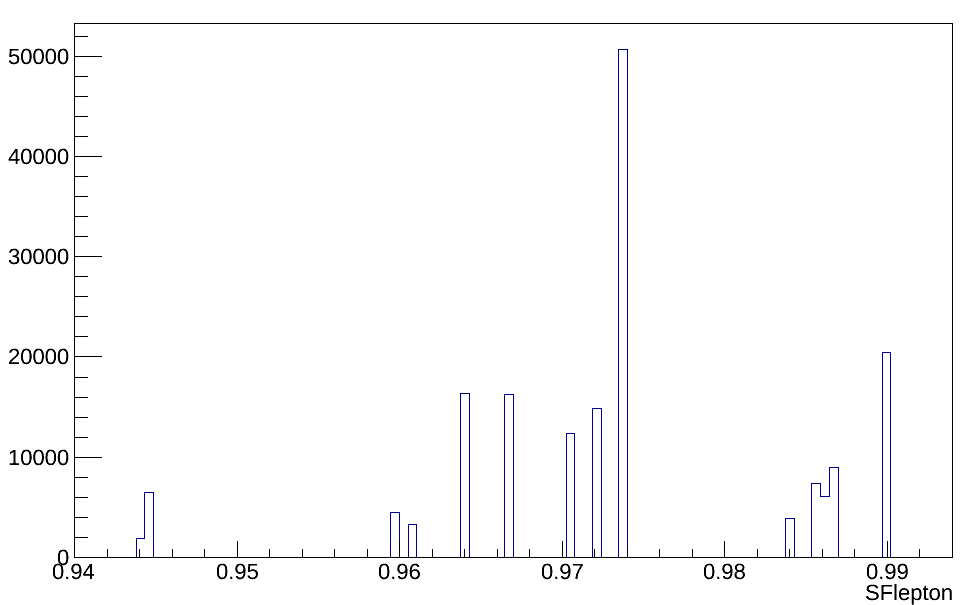
\includegraphics[width=0.45\textwidth]{images/Analysis/SFlepton.png}
    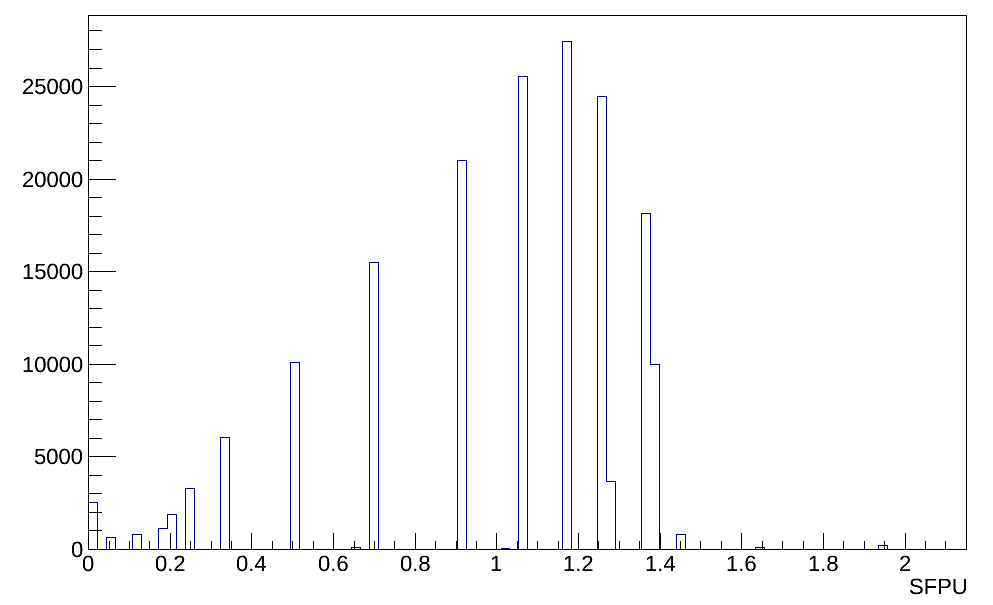
\includegraphics[width=0.45\textwidth]{images/Analysis/SFPU.png}
    \caption{Lepton SF (left) and PU SF (right).}
    \label{fig:SFs1}
\end{figure} 

\begin{figure}[ht]
\centering
    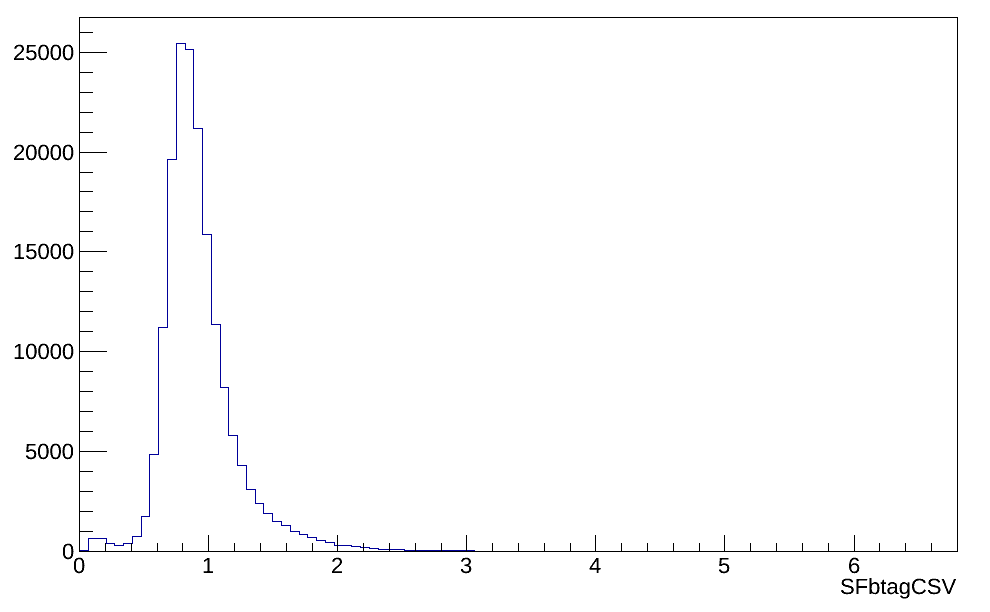
\includegraphics[width=0.45\textwidth]{images/Analysis/SFbtag.png}
    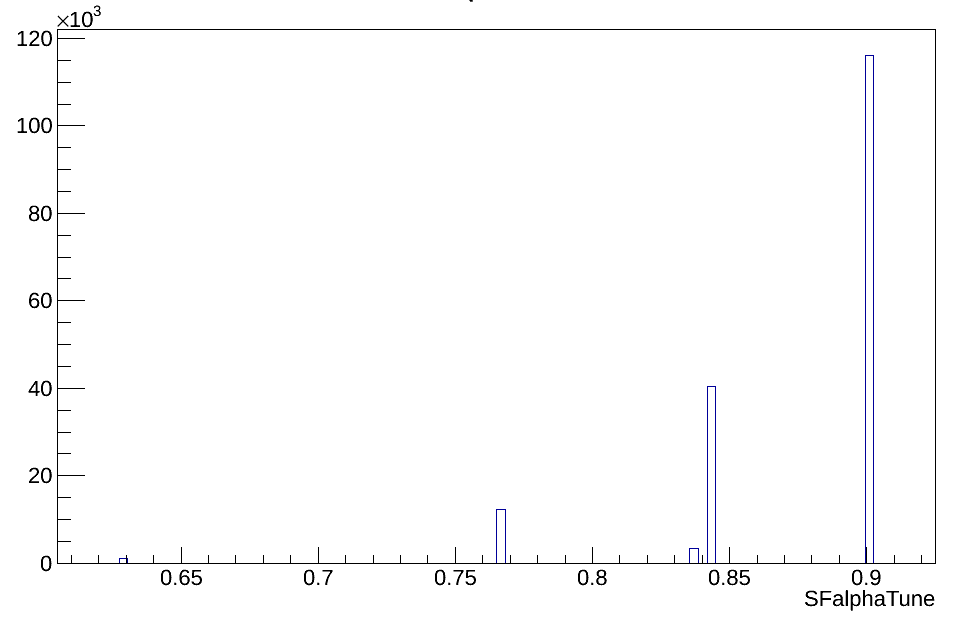
\includegraphics[width=0.45\textwidth]{images/Analysis/SFalpha.png}
    \caption{b-tag CSV SF (left) and jet modelling ($\alpha_S$) SF (right).}
    \label{fig:SFs2}
\end{figure} 

\section{Cross check on Multi-jet background estimation \label{app:MetReliso}}

% \section{\MET and Reliso}

Figure~\ref{fig:MetReliso} shows that there is no significant correlation between \MET and Reliso in \ttbar events.
\begin{figure}[ht]
\centering
    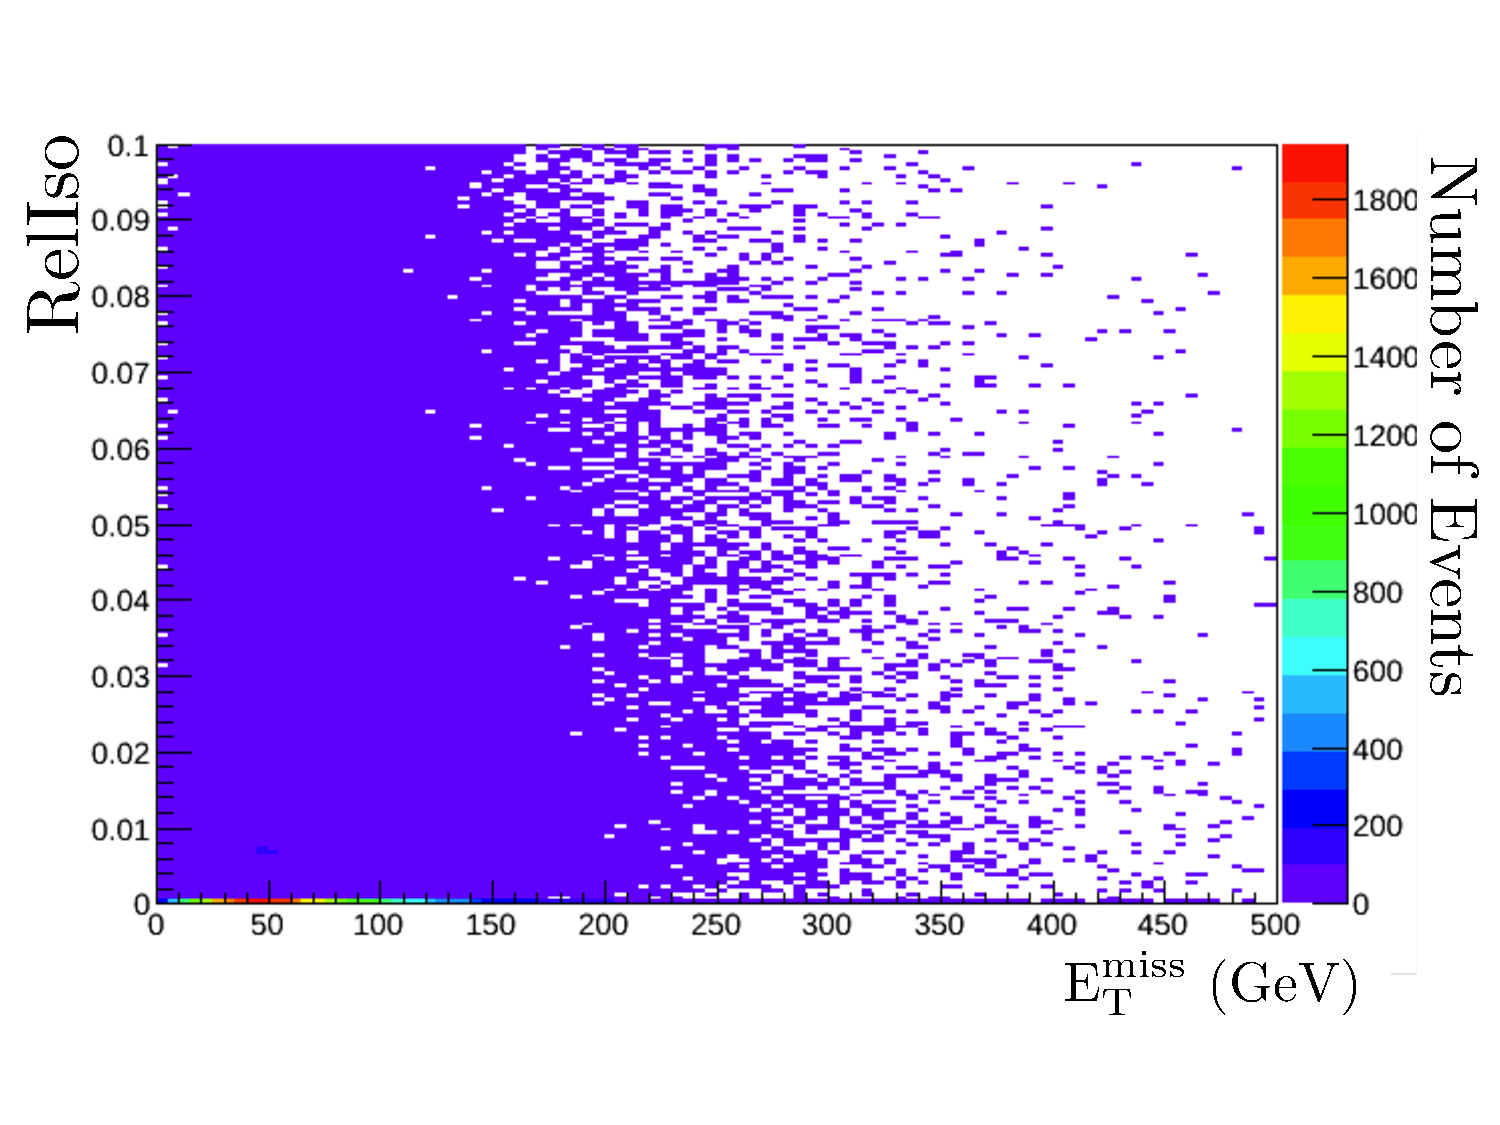
\includegraphics[width=0.7\textwidth]{images/Analysis/METreliso.pdf}
    \caption{\MET versus RelIso in \ttbar events.}
    \label{fig:MetReliso}
\end{figure} 

\chapter{Cross checks on \runone $\boldsymbol{\tttt}$ analysis at $\boldsymbol{\sqrt{s}=8}$~TeV \label{app:run1}}

\emph{This study was undertaken before the decision was made to split the BDT templates by the \njets categories.}

In the 2012 CMS differential cross-section \ttbar analysis \cite{CMS:TopPt} the \pt spectrum of top quarks tends towards higher values in the \MADGRAPH simulation than it is in data. Scale factors were derived by CMS to compensate for this effect. The analysis was performed with and without the application of the top \pt scale factors and the observed effect was negligible, as seen in Fig.~\ref{fig:studies8}, and hence these scale factors were not applied for the final result and no systematic uncertainty was included.\\
The uncertainty on the parton distribution functions (PDFs) are a potential source of systematic uncertainty. The method used by CMS to model this effect is given in~\cite{ref:PDFUnc2}. The BDT distributions which correspond to the maximal downward and upward fluctuation due to the uncertainty on the PDFs have a small effect on the shape of the BDT, as seen in Fig.~\ref{fig:studies8}, and are not considered further.\\
The uncertainty due to the choice of \PYTHIA tune used in the hadronisation of \ttbar events is considered. The nominal tune used is the $Z2^{*}$ tune which is compared to the alternative $P11$ tune~\cite{Khachatryan2011,Field:2011iq}. Again, there is a very small effect on the shape of the BDT, as seen in Fig.~\ref{fig:studies8}, so this uncertainty is not included in the final fit.

\begin{figure}[ht!]
\centering
    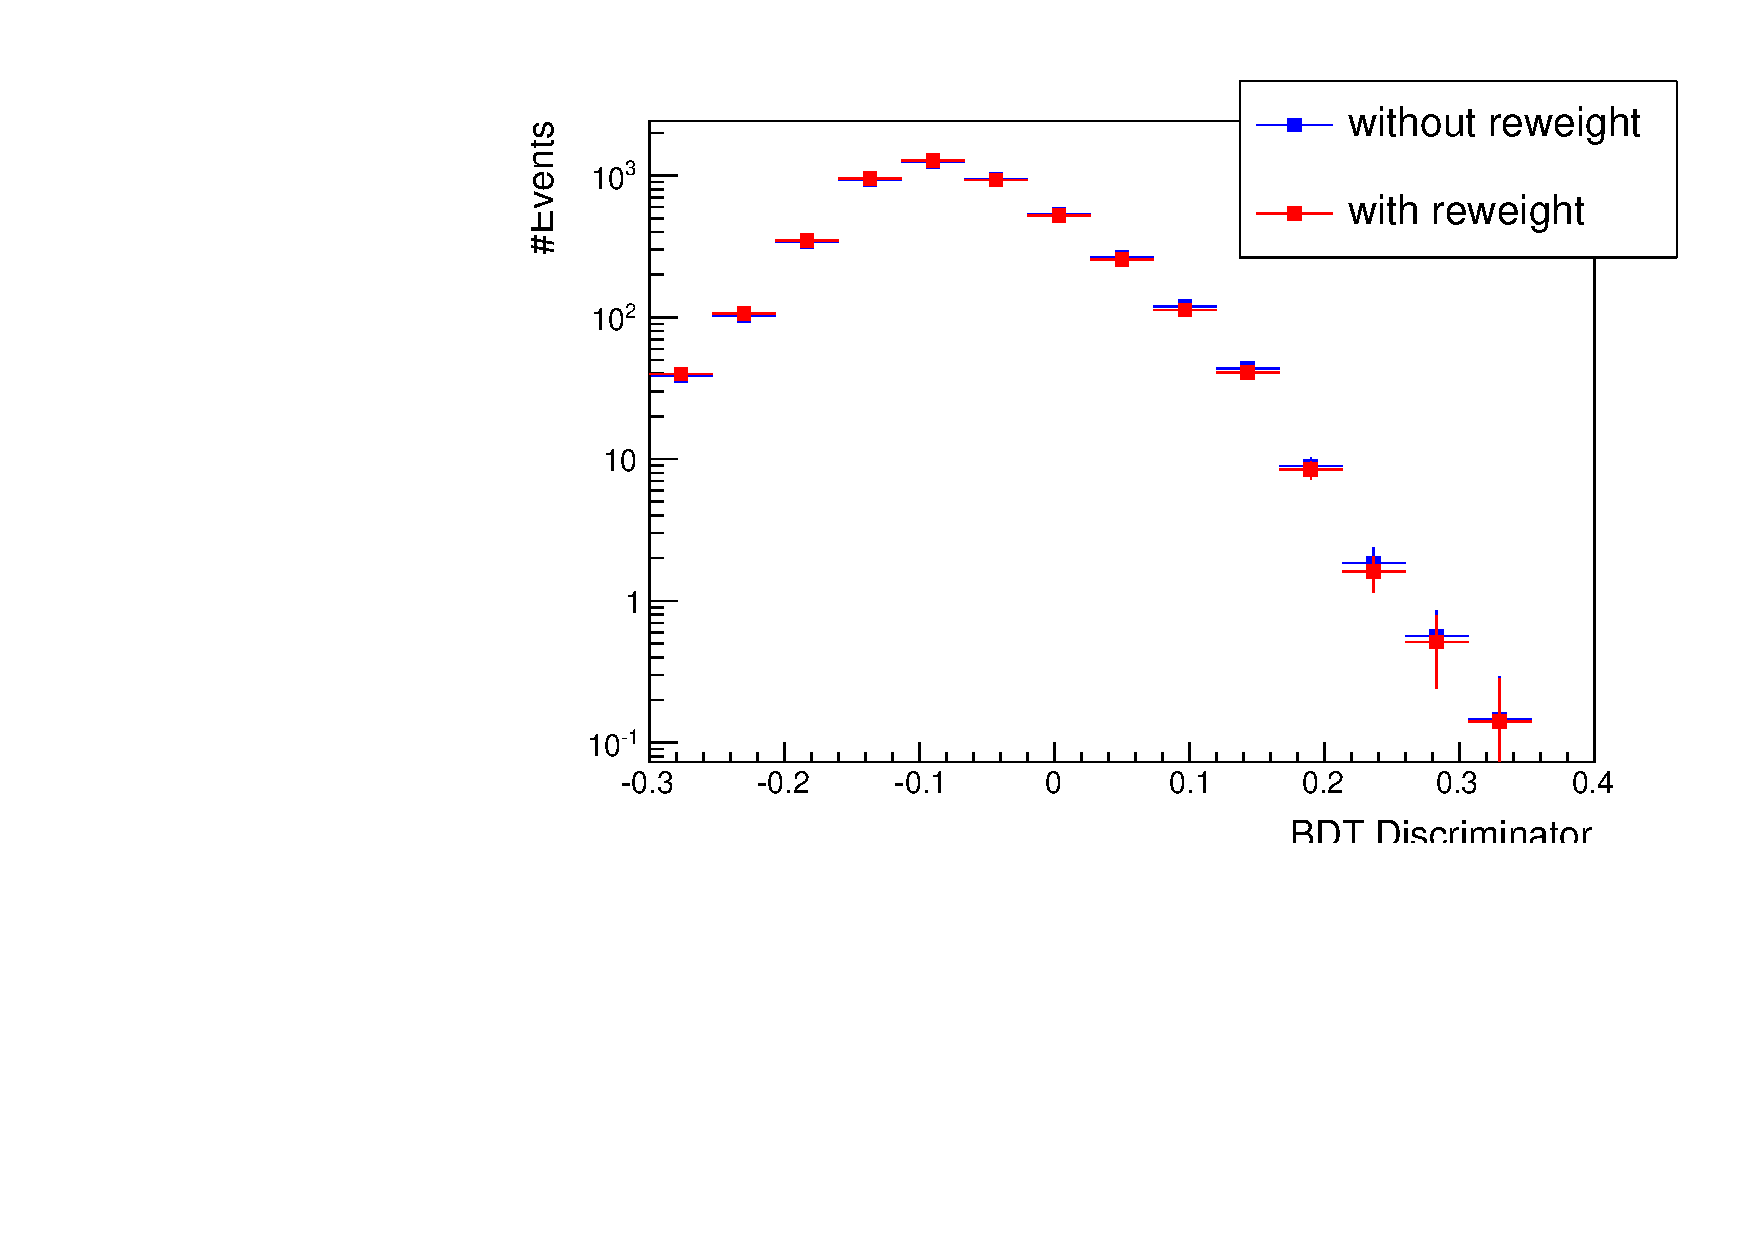
\includegraphics[width=0.49\textwidth]{images/Run1/ptrw_xcheck.pdf}
    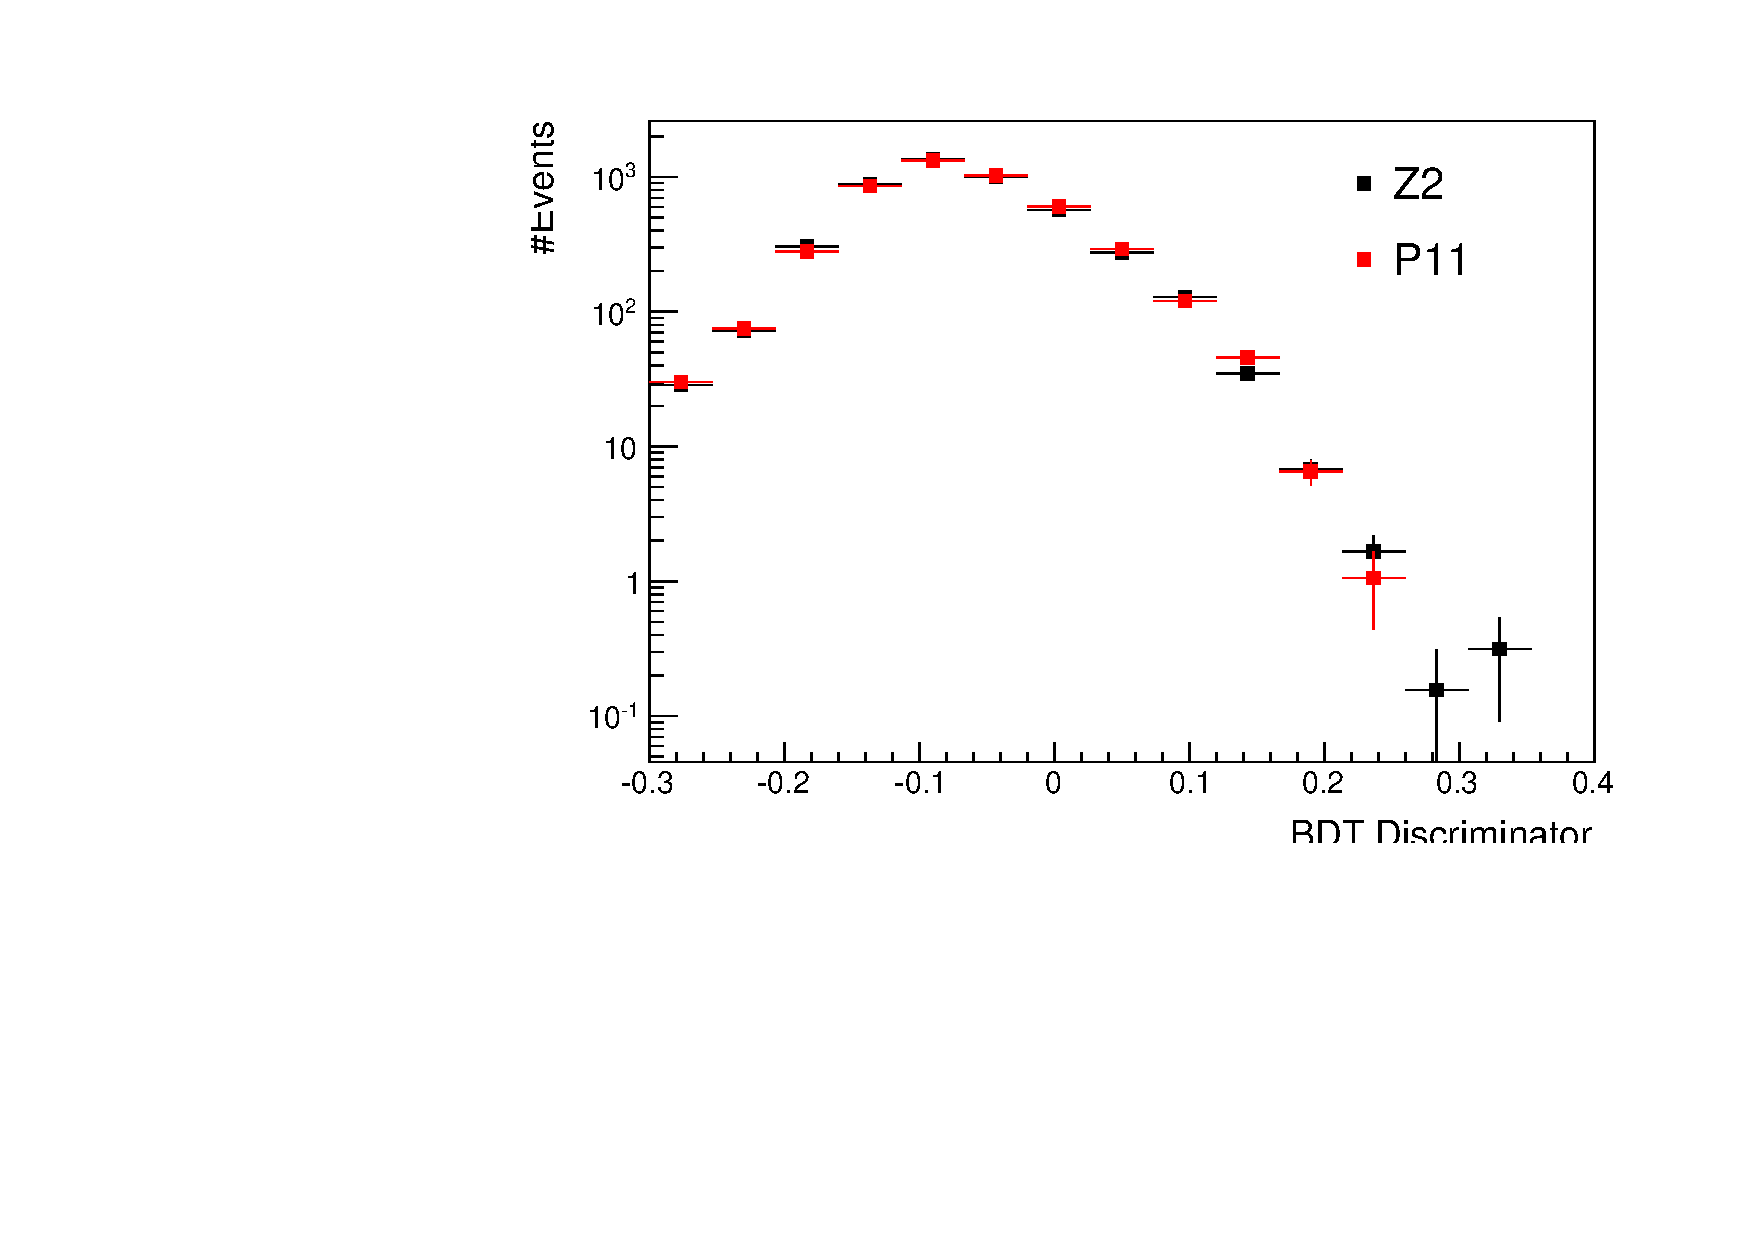
\includegraphics[width=0.49\textwidth]{images/Run1/NomTune_Mu_Log.pdf}\\
        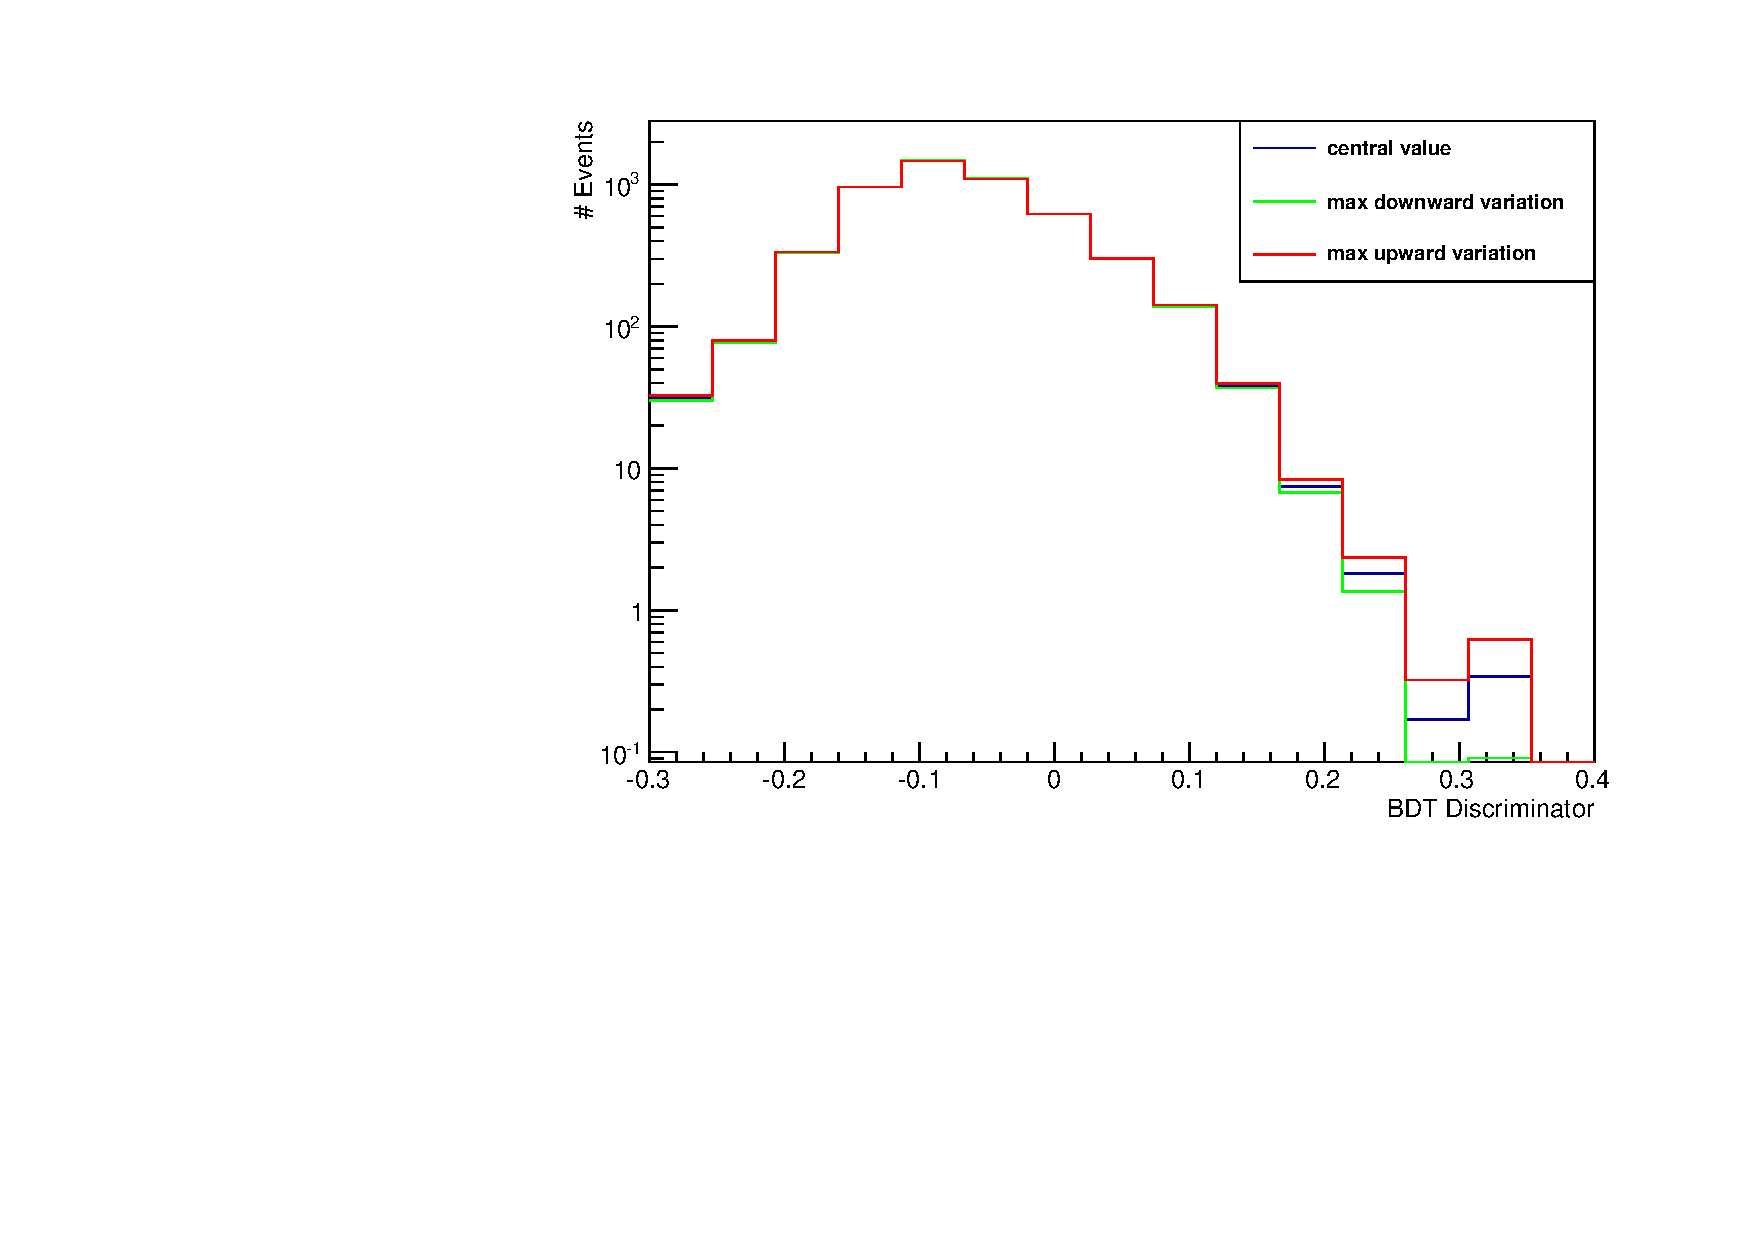
\includegraphics[width=0.7\textwidth]{images/Run1/PDF_uncertainty_mu.pdf}
    \caption{The BDT discriminator distributions of \ttbar simulation with and without the top quark \pt reweighting (top left), \PYTHIA tunes (top right) and PDF uncertainty (bottom).}
    \label{fig:studies8}
\end{figure}

\section{Cross-checks on the BDT \label{app:corplotsExc}}

Rankings of the input variables in terms of importance in the BDT are provided in tables \ref{tab:rankingmu} and \ref{tab:rankingel}, respectively.


\begin{table}[ht!]
\centering
\begin{tabular}{|c lc |c l p{3cm} |}
 \hline 
  Rank &   Variable & Variable Importance \\
  \hline   
1 & Jet6Pt   & 1.109e-01  \\
  \hline  
2 & HTX          & 1.092e-01 \\ 
  \hline  
  3 & MultiTopness          & 1.074e-01  \\
  \hline  
  4 & HTRat & 1.058e-01 \\  
  \hline  
 5 & HTb      & 1.003e-01  \\
  \hline  
6 & Jet5Pt        & 9.848e-02  \\ 
  \hline  
 7 & HTH  & 9.838e-02   \\
  \hline  
 8 & nJets       & 9.664e-02\\   
  \hline  
  9 & SumJetMassX        & 9.266e-02   \\
  \hline  
    10 & nTags        & 7.732e-02   \\
  \hline
\end{tabular}
\caption{The rankings of the input variables in terms of importance in the BDT for the $\mu$ + jets channel are provided. }
\label{tab:rankingmu}
\end{table}

\begin{table}[ht!]
\centering
\begin{tabular}{|c lc |c l p{3cm} |}
 \hline 
  Rank &   Variable & Variable Importance \\
  \hline   
 1 & MultiTopness          & 1.201e-01  \\
  \hline  
2 & HTRat         & 1.186e-01 \\ 
  \hline  
  3 & HTX          & 1.175e-01 \\
  \hline  
  4 & HTb        & 1.148e-01 \\  
  \hline  
  5 & HTH & 1.142e-01  \\
  \hline  
6 & Jet5Pt  & 9.730e-02  \\ 
  \hline  
7 & SumJetMassX     & 9.671e-02 \\
  \hline  
8 & Jet6Pt       & 8.913e-02\\   
  \hline  
  9 & nJets        & 7.319e-02   \\
  \hline  
    10 & nTags       & 5.850e-02   \\
  \hline 
  
\end{tabular}
\caption{The rankings of the input variables in terms of importance in the BDT for the $e$ + jets channel are provided. }
\label{tab:rankingel}
\end{table}




\chapter{Further detail on the phenomenological study in Chapter~\ref{c:pheno} \label{app:pheno}}

\section{Signal regions\label{app:pheno1}}

Figure~\ref{fig:SigReg} shows the signal regions defined in Ref.~\cite{Chatrchyan:2013fea}. These search regions are defined for high-\pt (lepton \pt$>$20~GeV) analyses and low-\pt analyses lepton \pt$>$10~GeV), the former of which is used in this thesis for SR28.

\begin{figure}[ht!]
\centering
    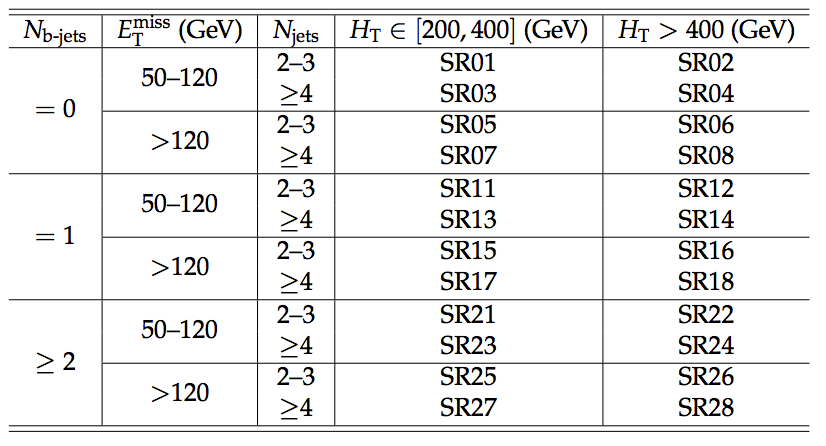
\includegraphics[width=\textwidth]{images/Pheno/SR28.png}
    \caption{Definition of the signal regions for the high-\pt analysis~\cite{Chatrchyan:2013fea}.}
    \label{fig:SigReg}
\end{figure}

Different combinations of these signal regions are used to provide ``broad coverage of strongly produced SUSY particles, including signatures with low hadronic activity as well as signatures involving third-generation squarks''~\cite{Chatrchyan:2013fea}.

\section{Parameterisation of the b-tagging of b-quark jets\label{app:pheno2}}

There is a small bump in the efficiency curve, shown in Fig~\ref{fig:effGraphs} (top-left). This is due to the parameterisation of the curve fitted from data. A polynomial of the form $Ax^3 + Bx^2 + Cx + D$ is used for $\pt<120$~GeV and a linear fit $Ex + F$ is used above that \pt threshold. The matching of these two function is the cause of the small bump in the curve and can also be seen in Ref.~\cite{Chatrchyan:2013fea}.
\begin{figure}[ht!]
\centering
    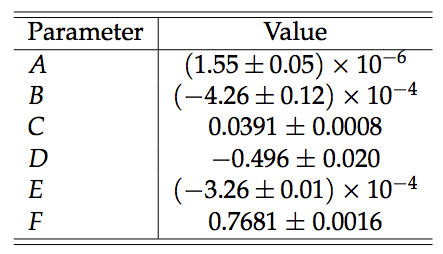
\includegraphics[width=0.45\textwidth]{images/Pheno/btageffparam.png}
    \caption{b-tagging efficiency parameters.}
    \label{fig:btageffparam}
\end{figure}

The efficiency functions for all efficiencies shown in Fig~\ref{fig:effGraphs} can be found in Ref.~\cite{Chatrchyan:2013fea}.

\chapter{Cross checks on \runtwo $\boldsymbol{\tttt}$ analysis at $\boldsymbol{\sqrt{s}=13}$~TeV}

% \section{Correlation matrices for fit nuisance parameters}


% \begin{figure}[ht!]
%     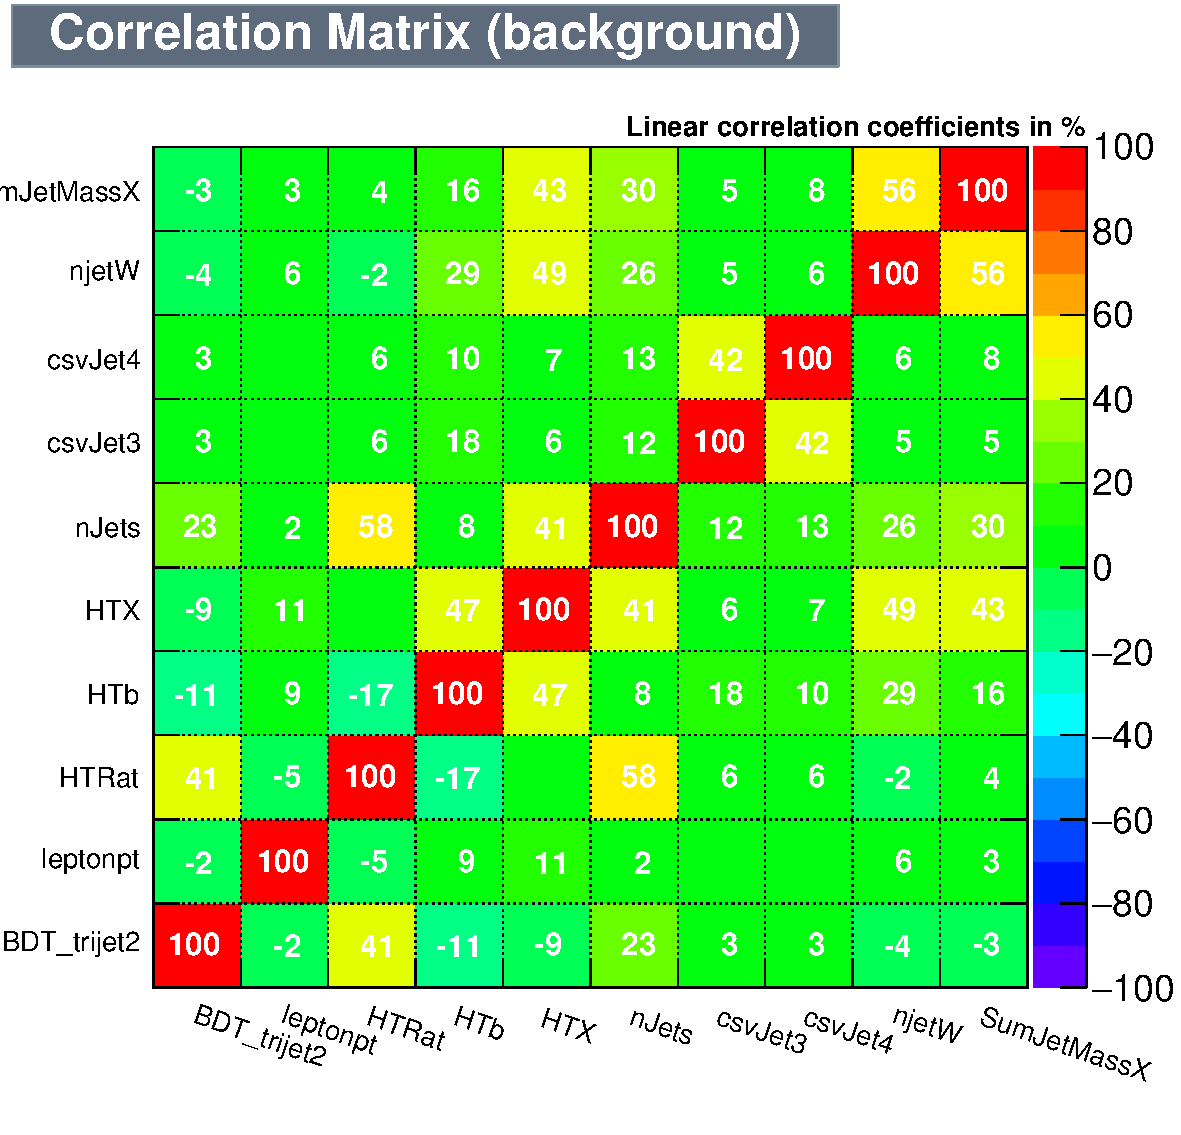
\includegraphics[width=0.48\textwidth]{images/Run2/CorrelationMatrixB.pdf}
%     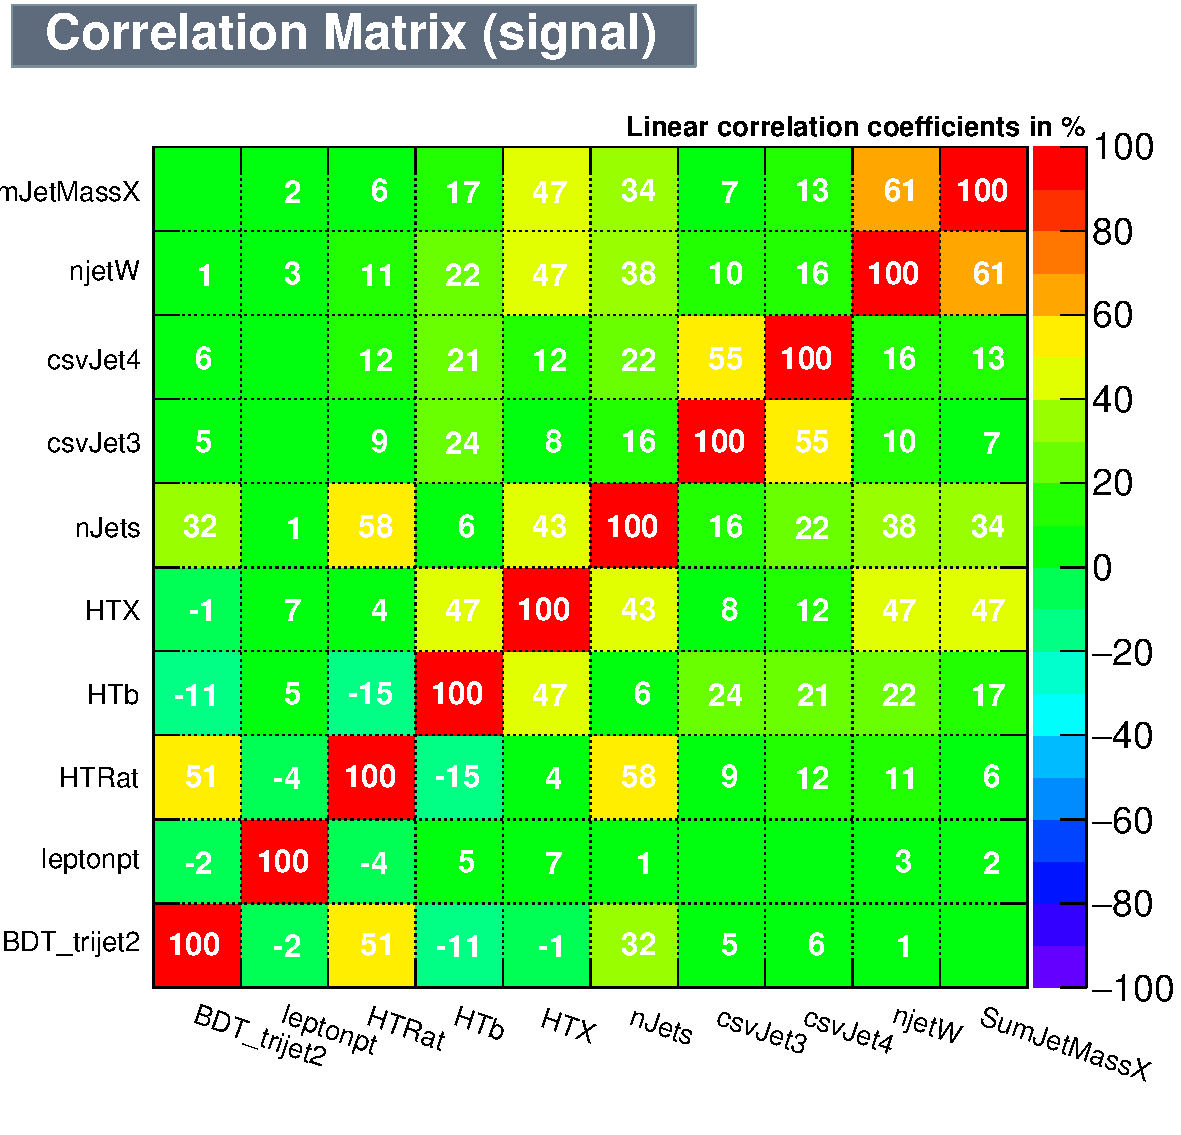
\includegraphics[width=0.48\textwidth]{images/Run2/CorrelationMatrixS.pdf}
%     \caption{The correlation matrices for background (left) and signal (right).}
%     \label{fig:corrMat}
% \end{figure}

% The correlation matrix for the fit nuisance parameters in the background only scenario can be see in Fig.~\ref{fig:FitCorr}. There is some correlation between the various b-tagging scale factors and also a correlation between the heavy flavour \heavyflavourone / \heavyflavourtwo modelling and the \ttbar ME scale, where the \heavyflavourone / \heavyflavourtwo is expected to be related to the choice of ME scale.

% \begin{figure}[ht!]
%     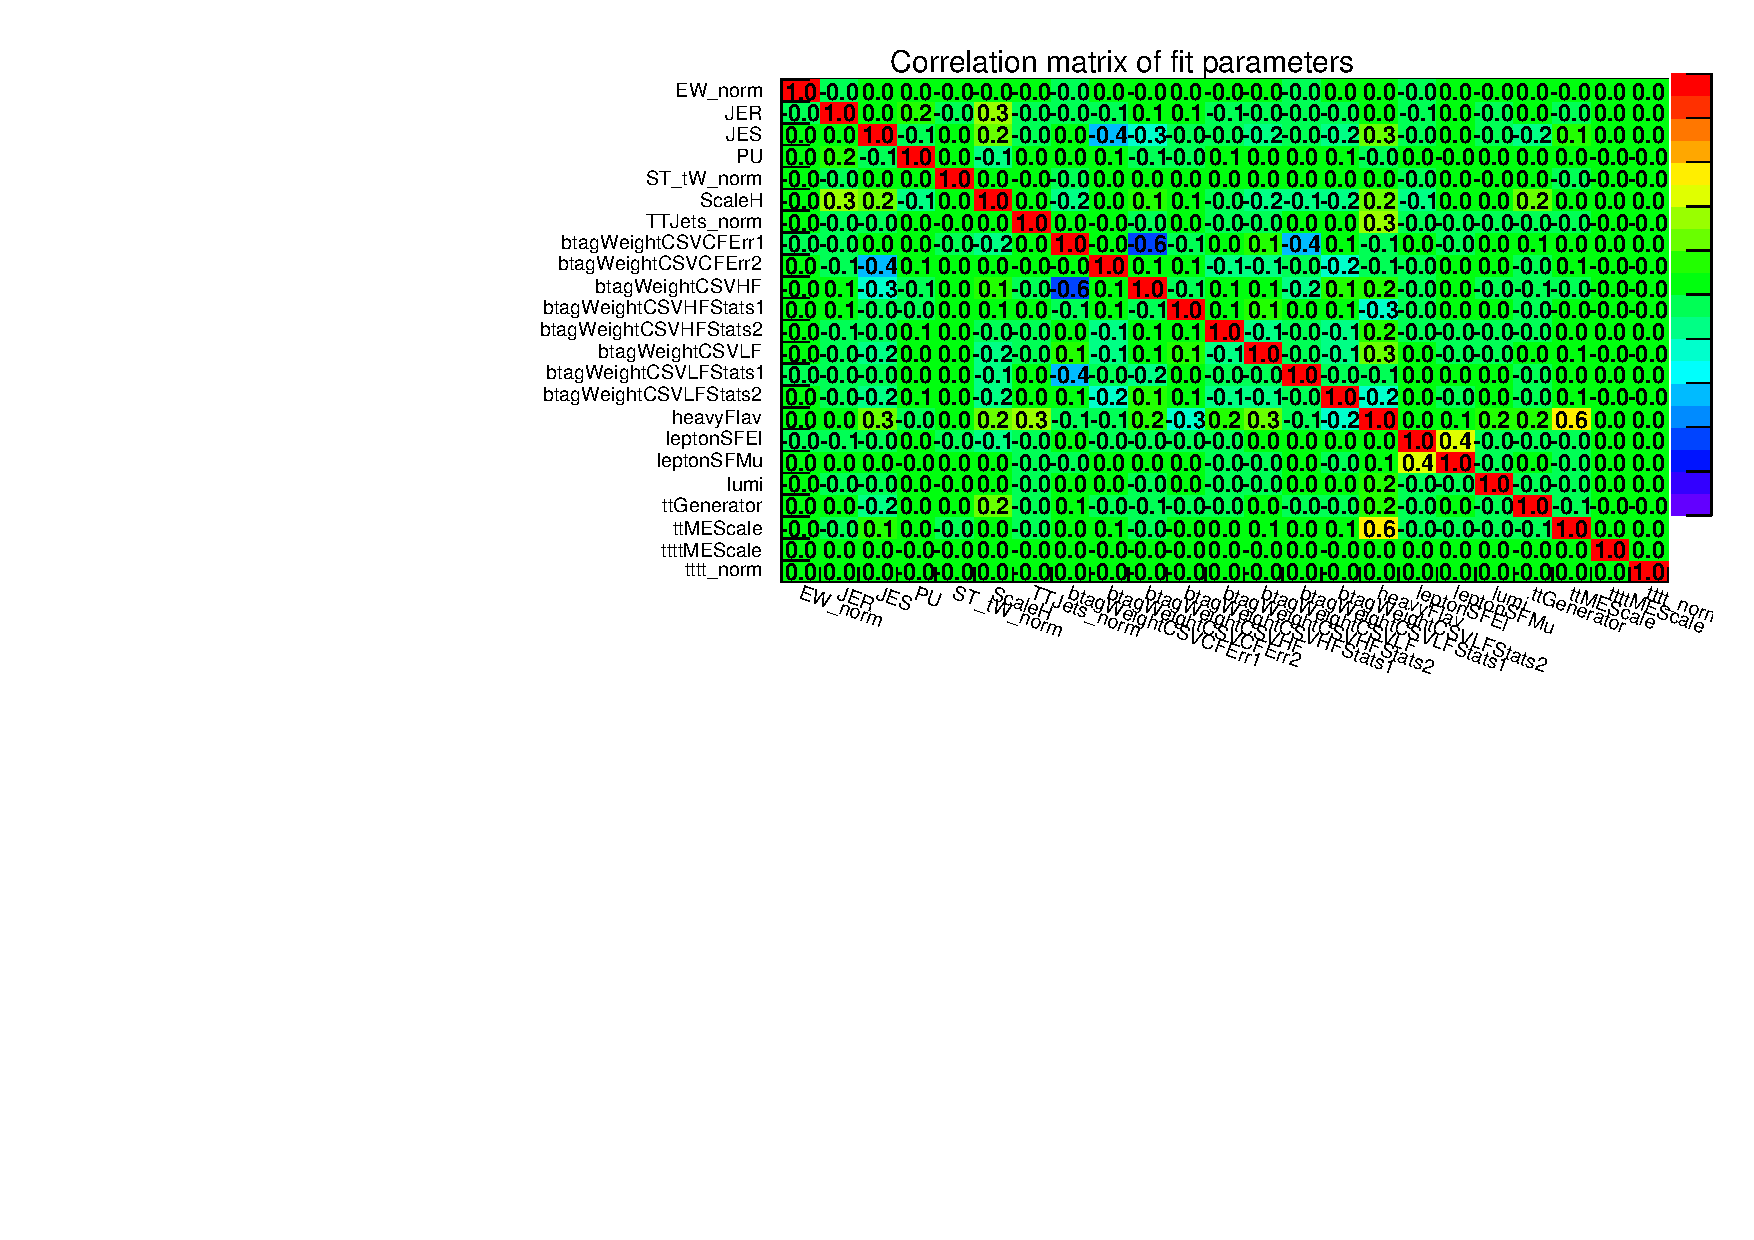
\includegraphics[width=0.9\textwidth]{images/Run2/FitCorr.pdf}
%     \caption{The correlation matrices for background only for the fit parameters.}
%     \label{fig:FitCorr}
% \end{figure}

\section{Comparison of alternative \ttbar generators \label{app:ttbargen}}

Figure~\ref{fig:MGFXFX} shows that the uncertainty from the \MADGRAPH \aMCATNLO generator is contained within the uncertainty from the \MLM generator, therefore it is conservative to use the \MLM generator as the systematic shape for differences in the BDT distribution due to generator choice.

\begin{figure}[ht]
\centering
    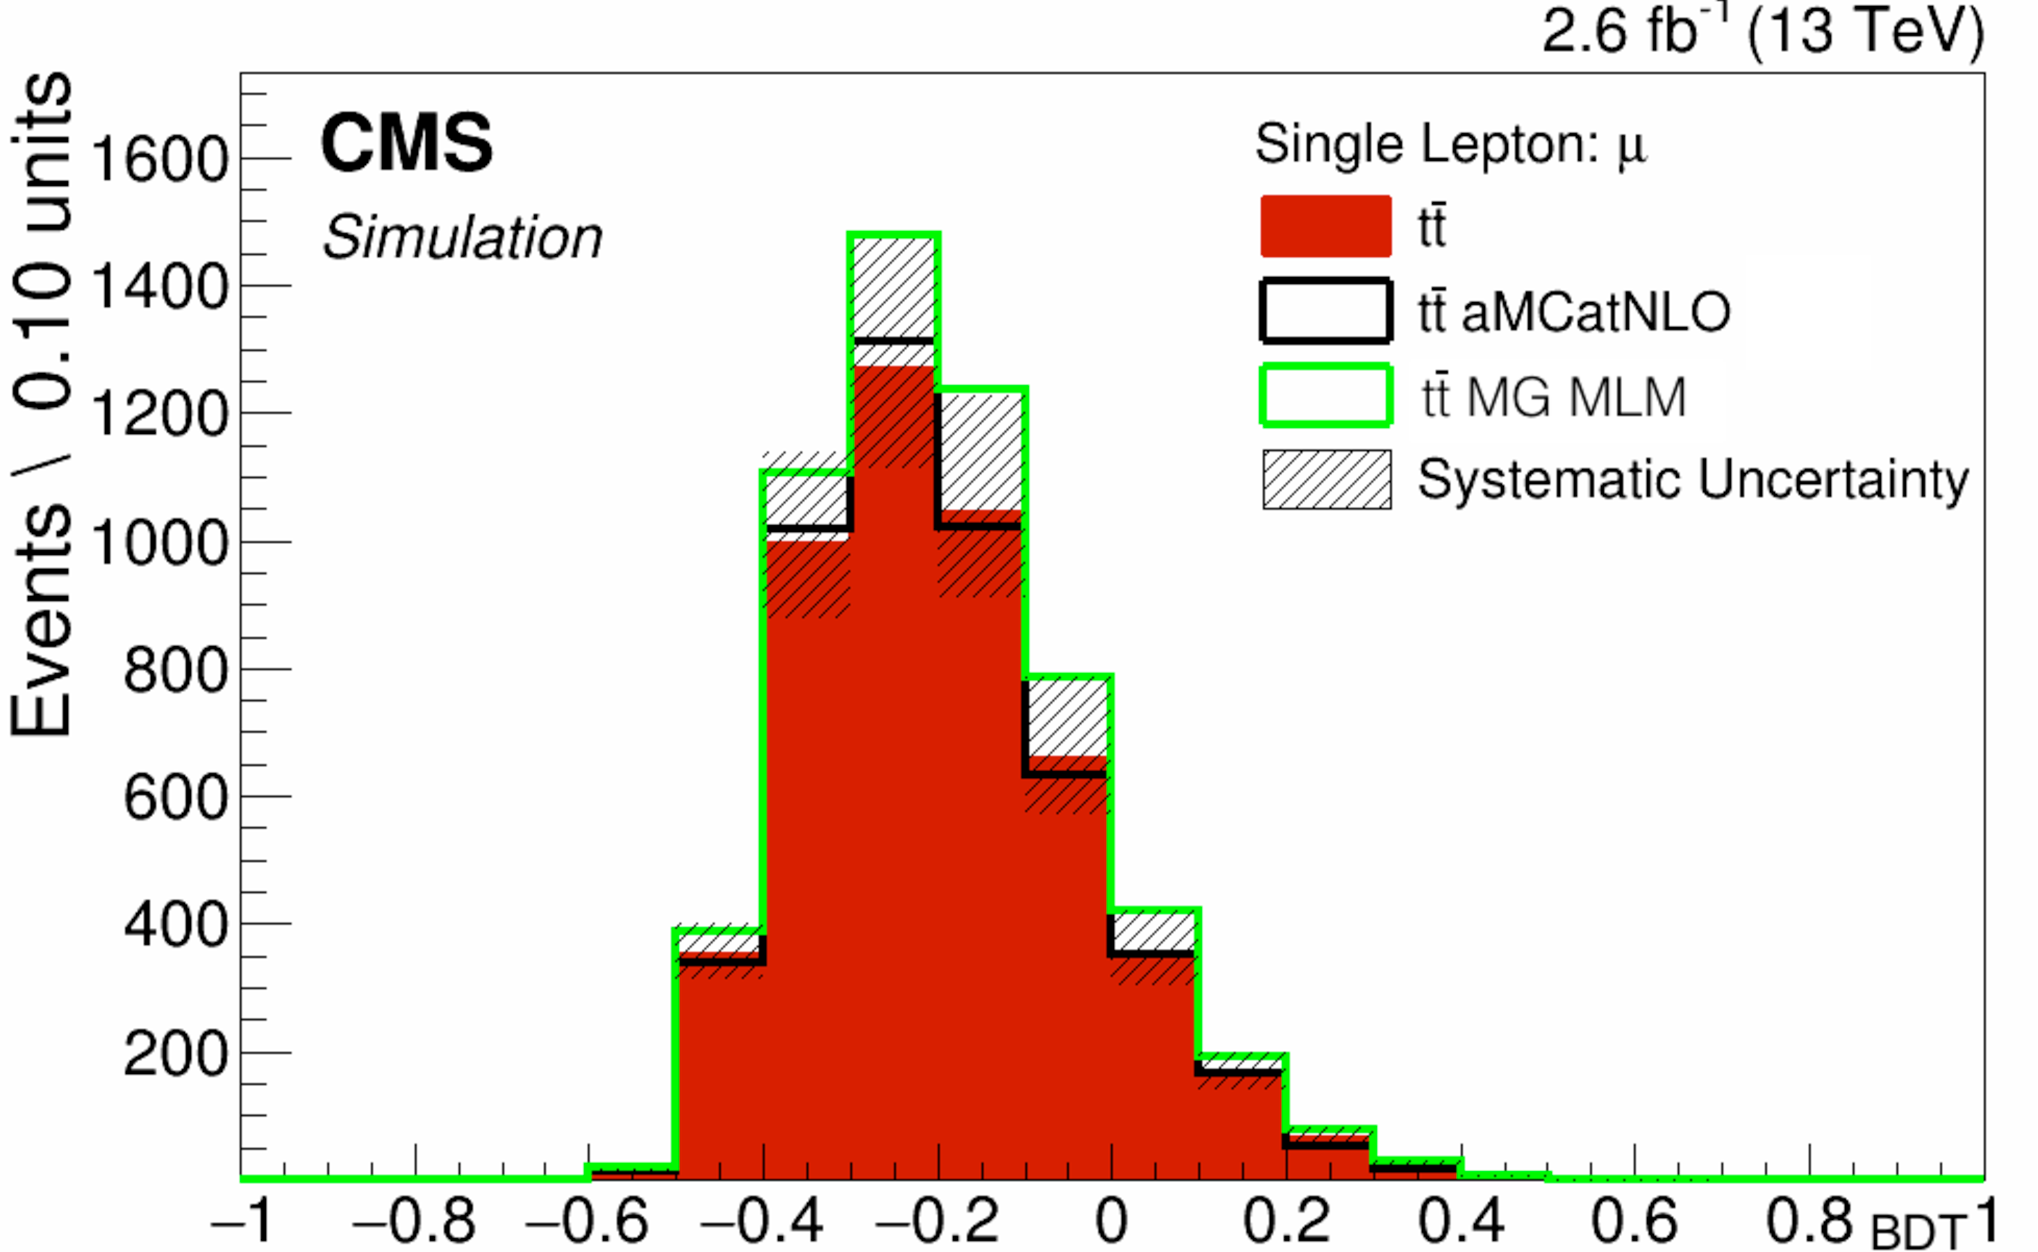
\includegraphics[width=0.7\textwidth]{images/Run2/MG_FXFX.pdf}
    \caption{Inclusive BDT distribution for \ttbar generators \POWHEG+\PYTHIA, \MLM and \MADGRAPH \aMCATNLO FxFx.}
    \label{fig:MGFXFX}
\end{figure} 



\section{TTZ, TTW, TTH MC backgrounds~\label{app:TTX}}
The contributions from \ttbar + B, where B = W, Z or H, were added to the predicted \ttbar yields to give a prediction for the net \ttbar + B background. The event-level BDT discriminant shapes for these contributions closely follow those of the \ttbar contribution and are very different from those predicted for the \tttt signal as a function of both the number of jets and the number of b-tagged jets. The differences are small and they over covered by the \ttbar scale uncertainties. Therefore, no additional systematic uncertainties were considered necessary to cover these backgrounds.


\begin{figure}[ht]
\centering
    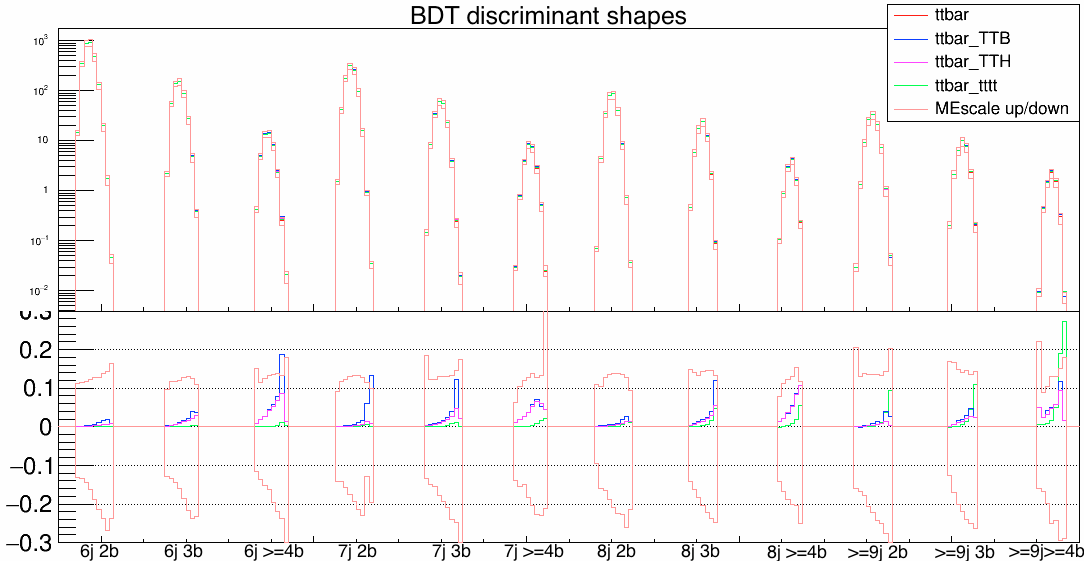
\includegraphics[width=\textwidth]{images/Run2/ttbarShapesLabels.png}
    \caption{BDT discriminator shapes for all categories, as indicated along the x axis. The ratio plot shows the difference between each distribution and the nominal \ttbar distribution divided by the \ttbar distribution.}
    \label{fig:TTB}
\end{figure}

\section{Comparison of the Gradient Boost and AdaBoost boosting algorithms within the BDT \label{app:gradBoost}}

For this study, the following three BDTs were trained:
\begin{enumerate}
\item \emph{GradNeg} - Gradient boosting taking into account negative weighting information in training and testing
\item \emph{GradBoost} - Gradient boosting ignoring negative weighting information in training and testing
\item \emph{AdaBoost} - AdaBoost boosting ignoring negative weighting information in training and testing
\end{enumerate}
% It was decided that if we were going to ignore the negative weight information then there was no reason to not include these events in the training sample. Additionally, if one was to ignore the negative weight information then there is no reason to not examine using AdaBoost.  
% Strategy 1 is referred to as \emph{GradNeg}; strategy 2 as \emph{GradBoost}; and strategy 3 as \emph{AdaBoost}. 
%
Each BDT was trained with the same set of input features and using the same sample of events to train and test the BDTs. The expected limits and uncertainties are shown for each strategy in Table~\ref{tab:BDTalgos} for the $\mu$ + jets and e + jets final states. Note that this study was performed at an earlier stage in the analysis so the results to do not correspond exactly to the final expected limit given in Section~\ref{sec:limit13}. The BDT output discriminator distribution was only split into \njets categories of of 6, 7, 8, 9+ jets at this stage rather than \njets and \nMtags categories.
 % The response of the signal and background samples as well as the ROC curves for the derived classifiers for each strategy can be seen in Figs. \ref{fig:GradNeg} through \ref{fig:AdaBoost}.



\begin{table}[ht]
\centering
\caption{Expected limits using jet categories of 6, 7, 8, 9+ jets for different BDT boosting algorithms.}
\label{tab:BDTalgos}
\begin{tabular}{|l|l|l|l|l|}
\hline
Algorithm & $\mu$ + jets & uncertainty & e + jets & uncertainty \\ \hline
GradNeg   & 18.1         & +8.0, -5.3  & 27.6     & +12.9, -8.3 \\ \hline
GradBoost & 18.7         & +8.3, -5.5  & 28.8     & +12.9, -8.3 \\ \hline
AdaBoost  & 10.7         & +6.4, -4.0  & 21.6     & +10.9, -7.0 \\ \hline
\end{tabular}
\end{table}

It can be seen from Table~\ref{tab:BDTalgos} that the difference between including negative weight information in the GradNeg strategy and not including it in the GradBoost strategy have a negligible effect on the expected limit within the uncertainties. Using negative weights may slightly optimise the modelling for training but not significantly hence the AdaBoost strategy can be used without negative weights as it has a significant benefit in lowering the expected limit.


\section{Event-level BDT templates \label{app:BDTtemp}}


\begin{figure}[ht!]
    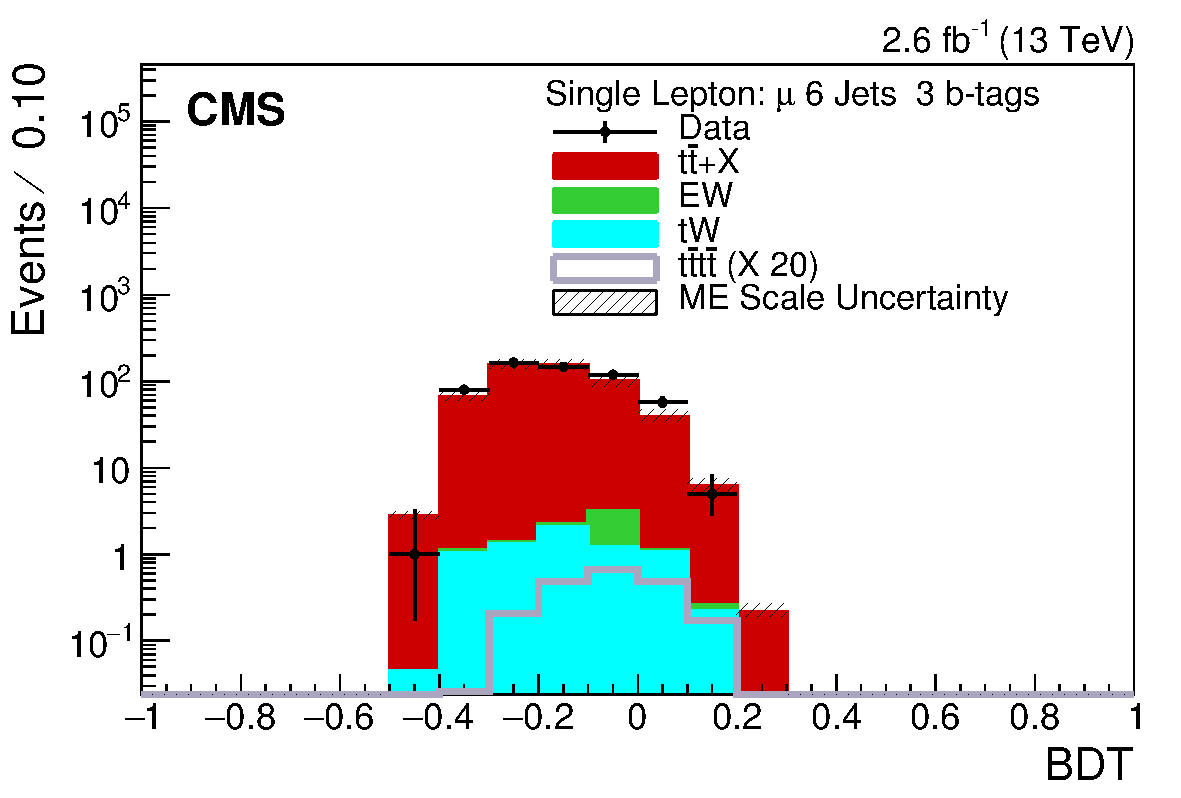
\includegraphics[width=0.48\textwidth]{images/Run2/BDT_Mu29Aug400trees_5MinNodeSize_20nCuts_3MaxDepth_5adaboostbeta_adaBoost_alphaSTune_noMinEvents6nJets3nMtags_StackLogY.pdf}
    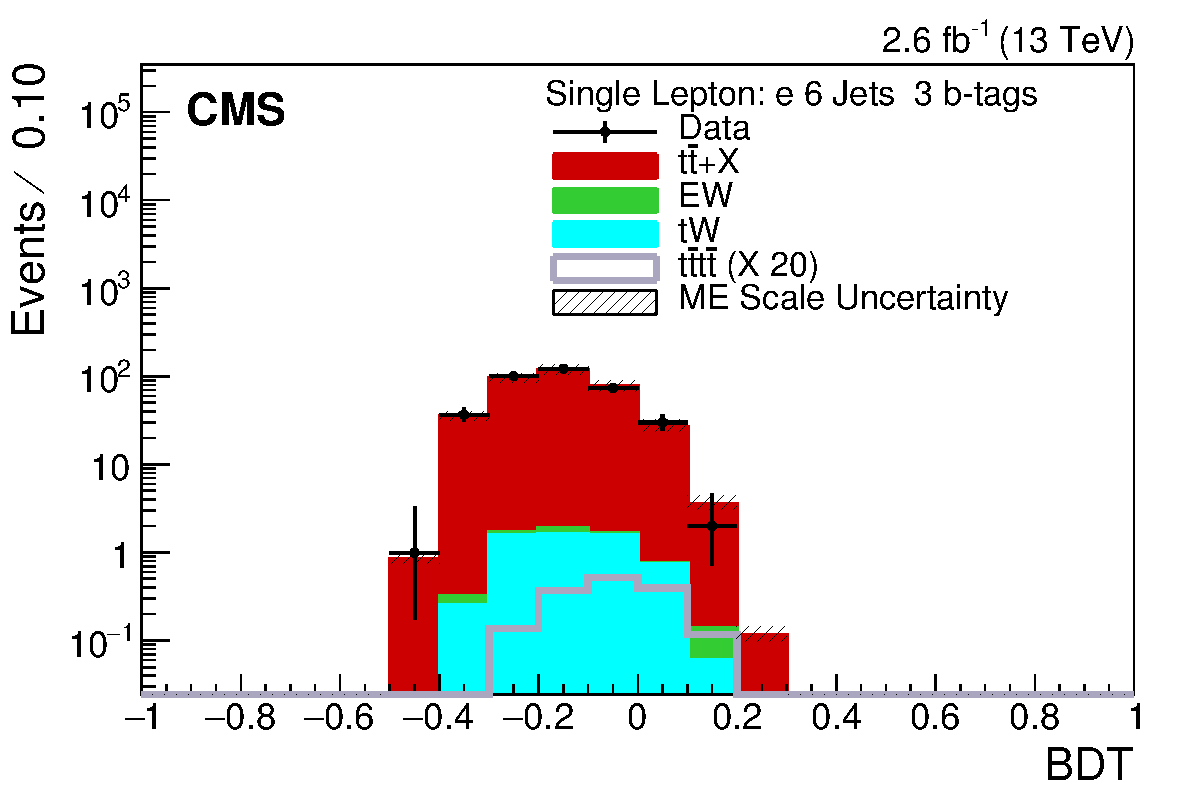
\includegraphics[width=0.48\textwidth]{images/Run2/BDT_El29Aug400trees_5MinNodeSize_20nCuts_3MaxDepth_5adaboostbeta_adaBoost_alphaSTune_noMinEvents6nJets3nMtags_StackLogY.pdf} 
    \caption{The BDT output distributions for AdaBoost for data and simulation in the $\mu$ + jets channel (left) and e + jets channel (left) are shown for the 6 \njets and 3\nMtags category.}
    \label{fig:BDT_Mu29Aug400trees_5MinNodeSize_20nCuts_3MaxDepth_5adaboostbeta_adaBoost_alphaSTune_noMinEvents63}
\end{figure}

\begin{figure}[ht!]
    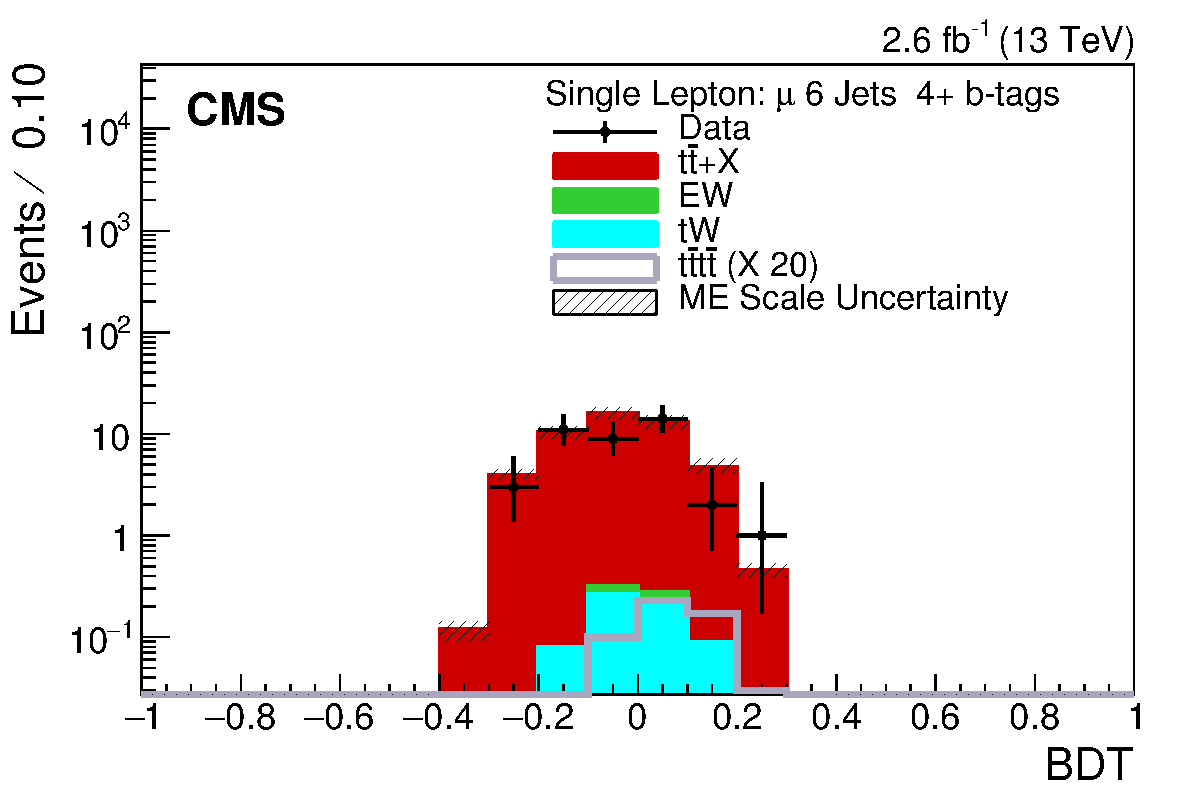
\includegraphics[width=0.48\textwidth]{images/Run2/BDT_Mu29Aug400trees_5MinNodeSize_20nCuts_3MaxDepth_5adaboostbeta_adaBoost_alphaSTune_noMinEvents6nJets4nMtags_StackLogY.pdf}
    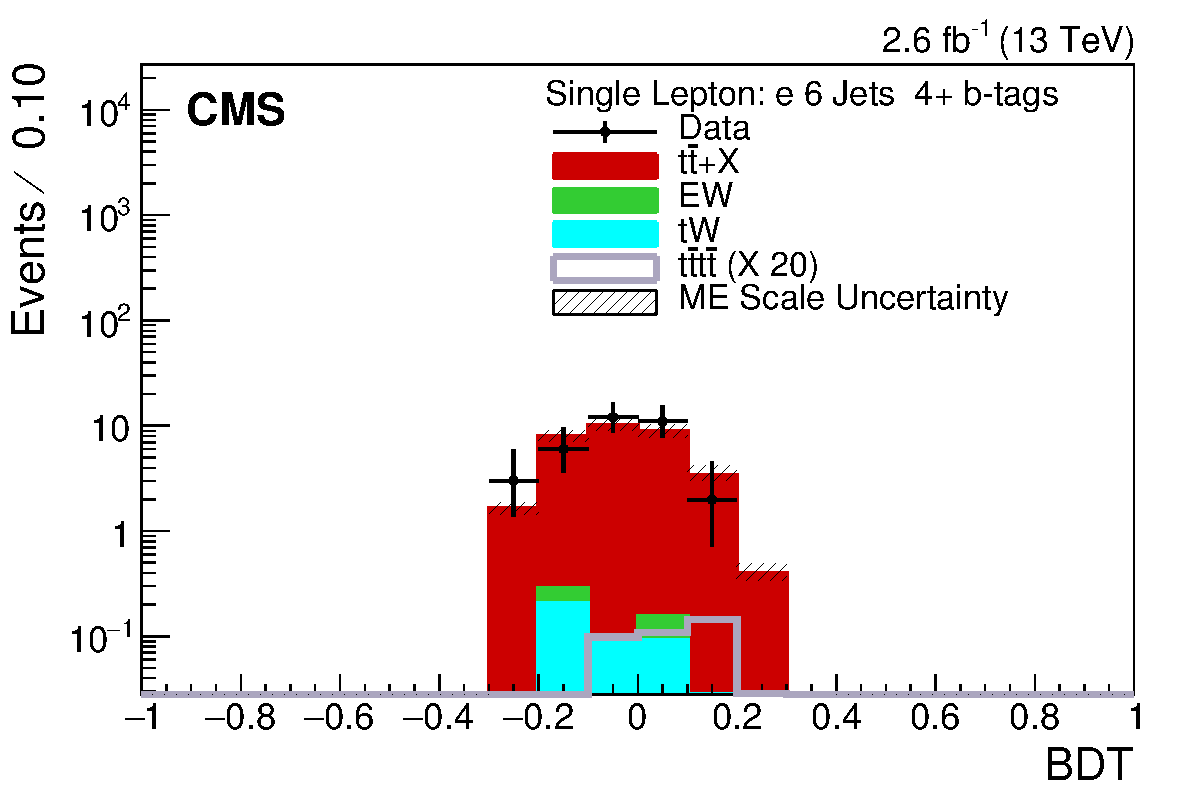
\includegraphics[width=0.48\textwidth]{images/Run2/BDT_El29Aug400trees_5MinNodeSize_20nCuts_3MaxDepth_5adaboostbeta_adaBoost_alphaSTune_noMinEvents6nJets4nMtags_StackLogY.pdf}
    \caption{The BDT output distributions for AdaBoost for data and simulation in the $\mu$ + jets channel (left) and e + jets channel (right) are shown for the 6 \njets and $\geq4$ \nMtags category.}
    \label{fig:BDT_Mu29Aug400trees_5MinNodeSize_20nCuts_3MaxDepth_5adaboostbeta_adaBoost_alphaSTune_noMinEvents64}
\end{figure}

\begin{figure}[ht!]
    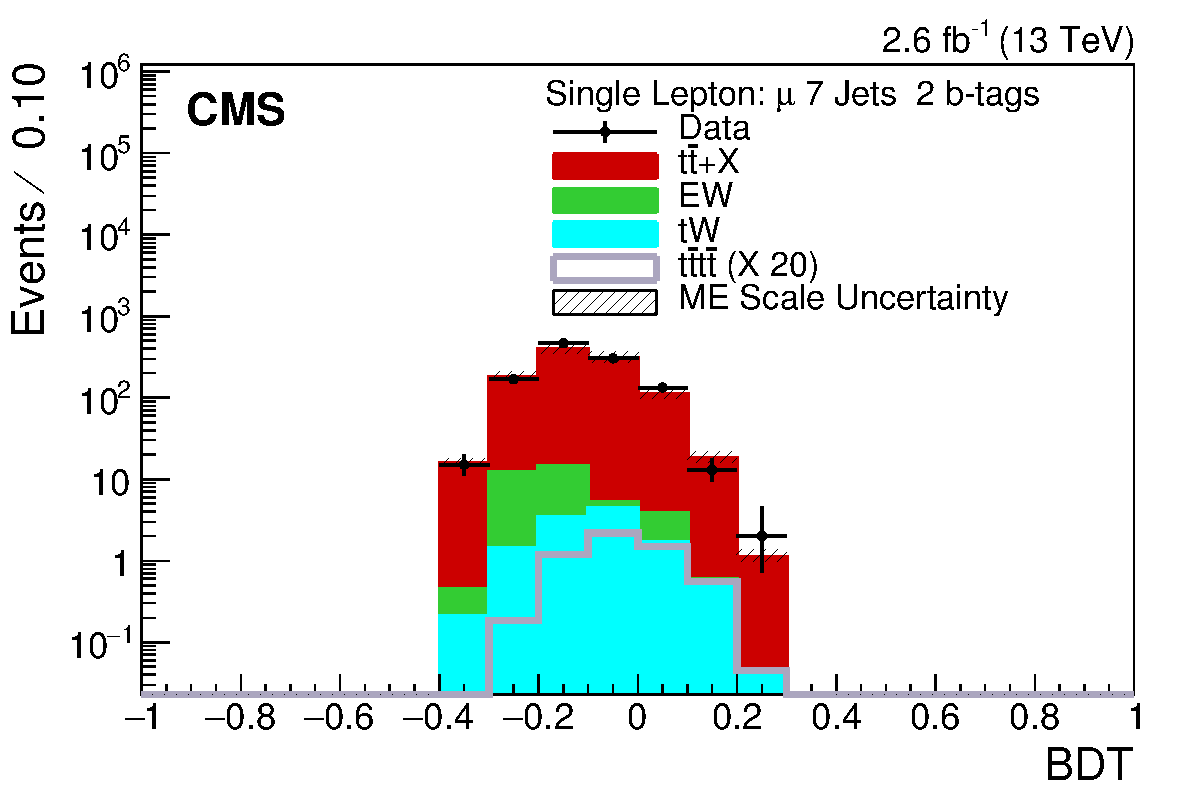
\includegraphics[width=0.48\textwidth]{images/Run2/BDT_Mu29Aug400trees_5MinNodeSize_20nCuts_3MaxDepth_5adaboostbeta_adaBoost_alphaSTune_noMinEvents7nJets2nMtags_StackLogY.pdf}
    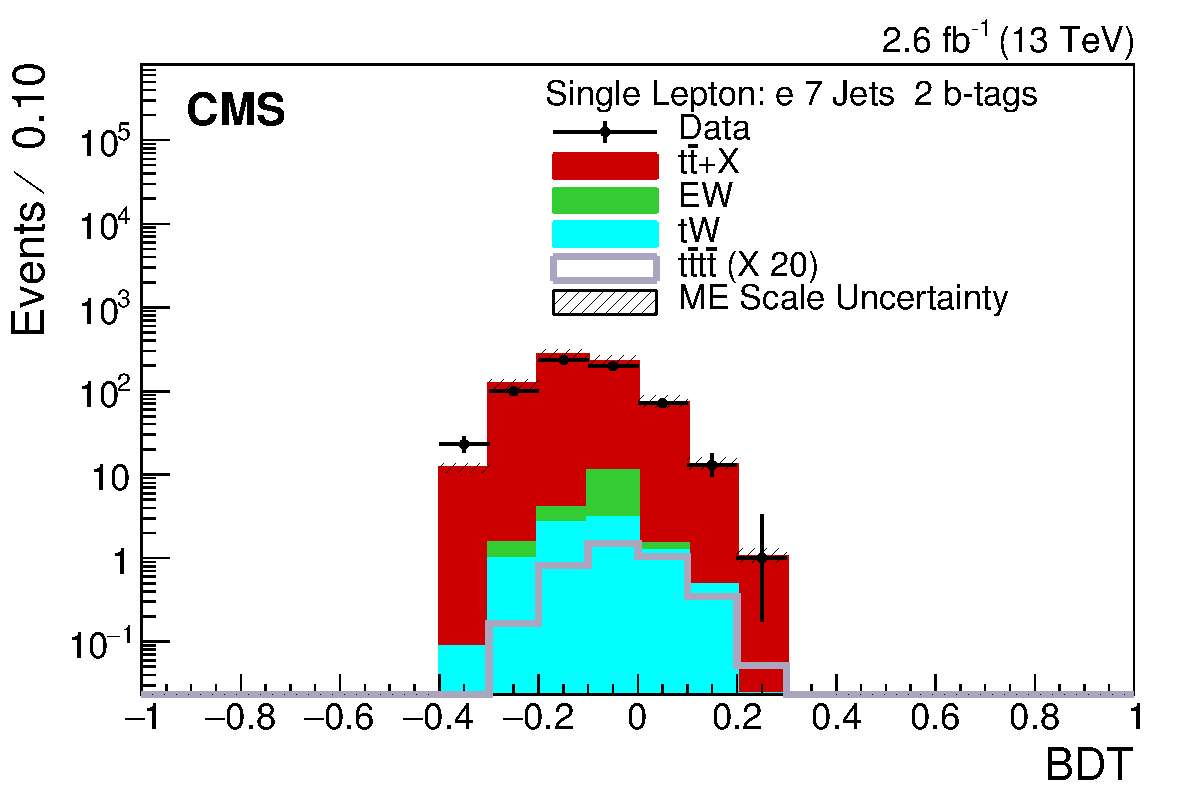
\includegraphics[width=0.48\textwidth]{images/Run2/BDT_El29Aug400trees_5MinNodeSize_20nCuts_3MaxDepth_5adaboostbeta_adaBoost_alphaSTune_noMinEvents7nJets2nMtags_StackLogY.pdf} 
    \caption{The BDT output distributions for AdaBoost for data and simulation in the $\mu$ + jets channel (left) and e + jets channel (left) are shown for the 7 \njets and 2 \nMtags category.}
    \label{fig:BDT_Mu29Aug400trees_5MinNodeSize_20nCuts_3MaxDepth_5adaboostbeta_adaBoost_alphaSTune_noMinEvents72}
 \end{figure}

\begin{figure}[ht!]
    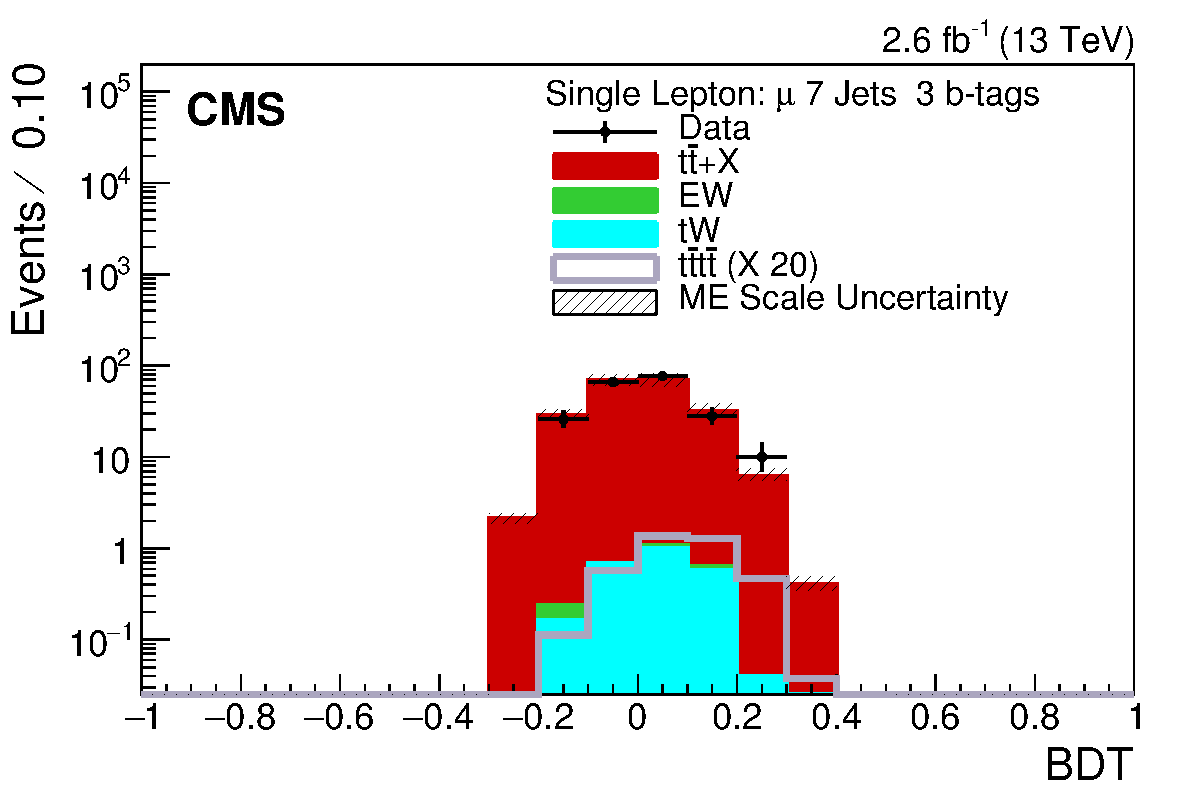
\includegraphics[width=0.48\textwidth]{images/Run2/BDT_Mu29Aug400trees_5MinNodeSize_20nCuts_3MaxDepth_5adaboostbeta_adaBoost_alphaSTune_noMinEvents7nJets3nMtags_StackLogY.pdf}
    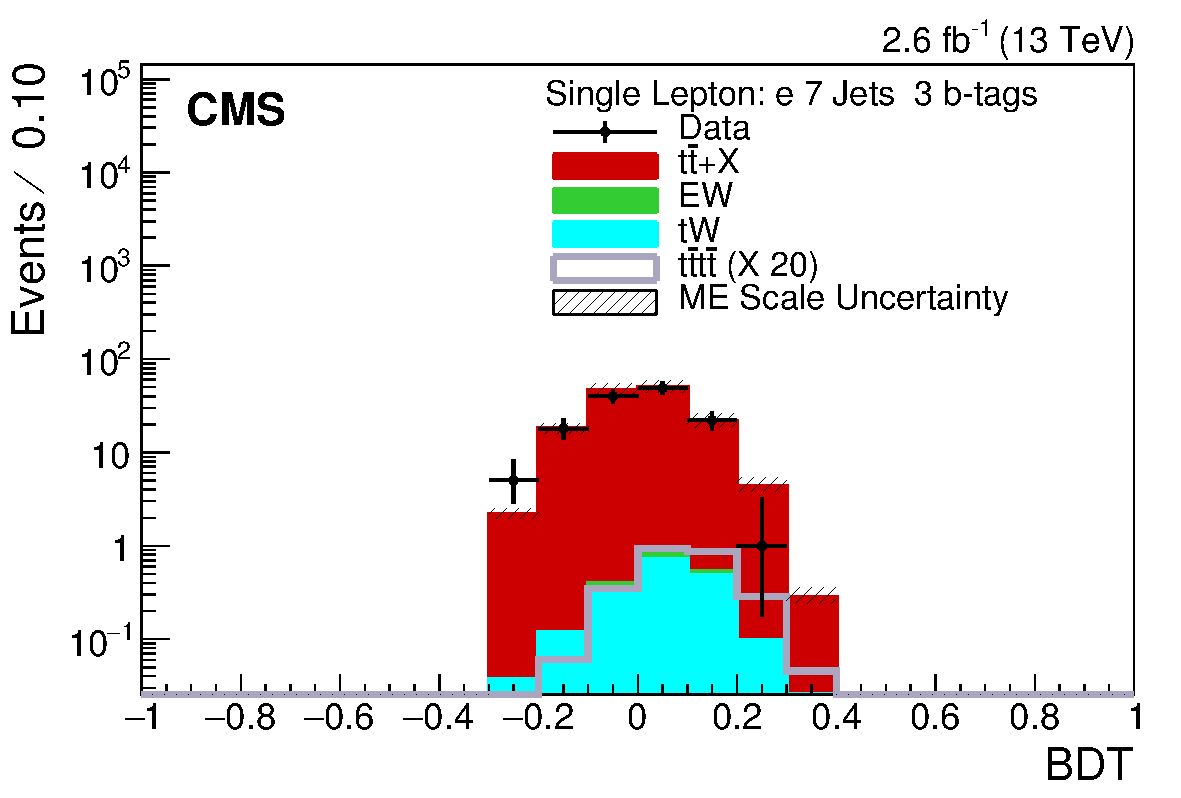
\includegraphics[width=0.48\textwidth]{images/Run2/BDT_El29Aug400trees_5MinNodeSize_20nCuts_3MaxDepth_5adaboostbeta_adaBoost_alphaSTune_noMinEvents7nJets3nMtags_StackLogY.pdf}
    \caption{The BDT output distributions for AdaBoost for data and simulation in the $\mu$ + jets channel (left) and e + jets channel (left) are shown for the 7 \njets and 3 \nMtags category.}
    \label{fig:BDT_Mu29Aug400trees_5MinNodeSize_20nCuts_3MaxDepth_5adaboostbeta_adaBoost_alphaSTune_noMinEvents73}
 \end{figure}

\begin{figure}[ht!]
    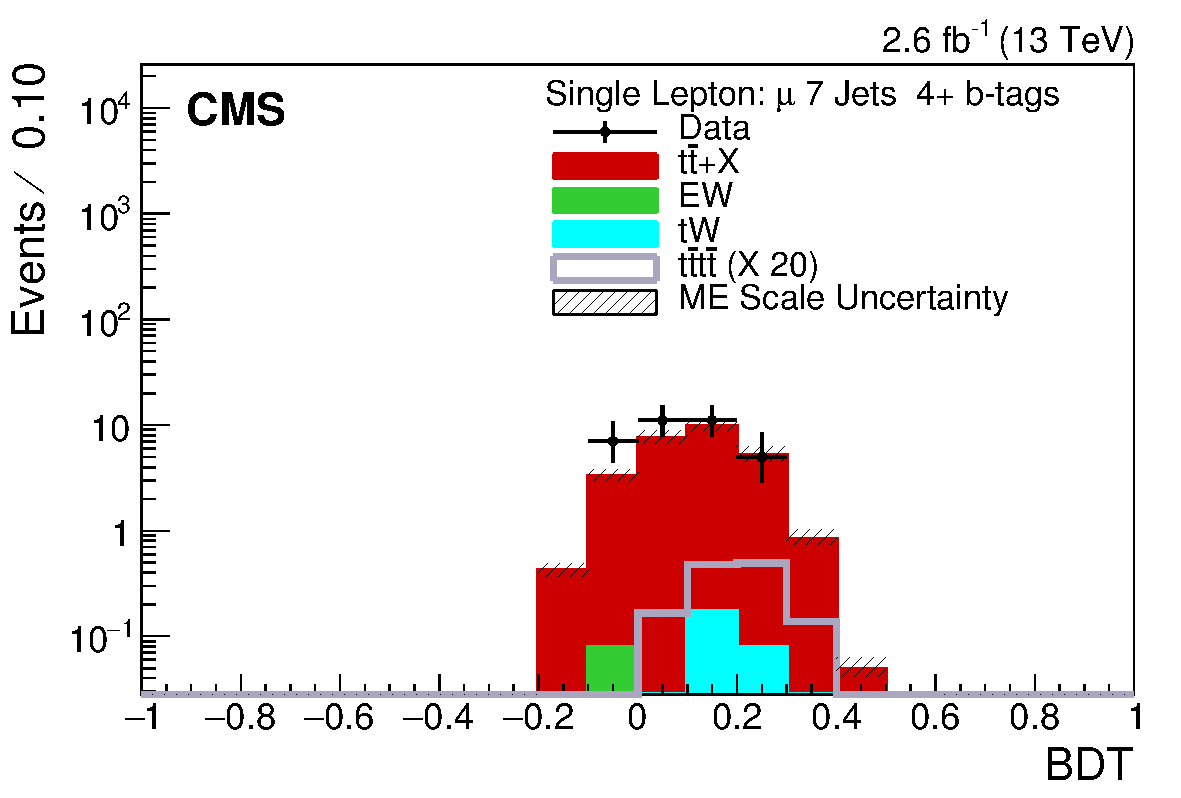
\includegraphics[width=0.48\textwidth]{images/Run2/BDT_Mu29Aug400trees_5MinNodeSize_20nCuts_3MaxDepth_5adaboostbeta_adaBoost_alphaSTune_noMinEvents7nJets4nMtags_StackLogY.pdf}
    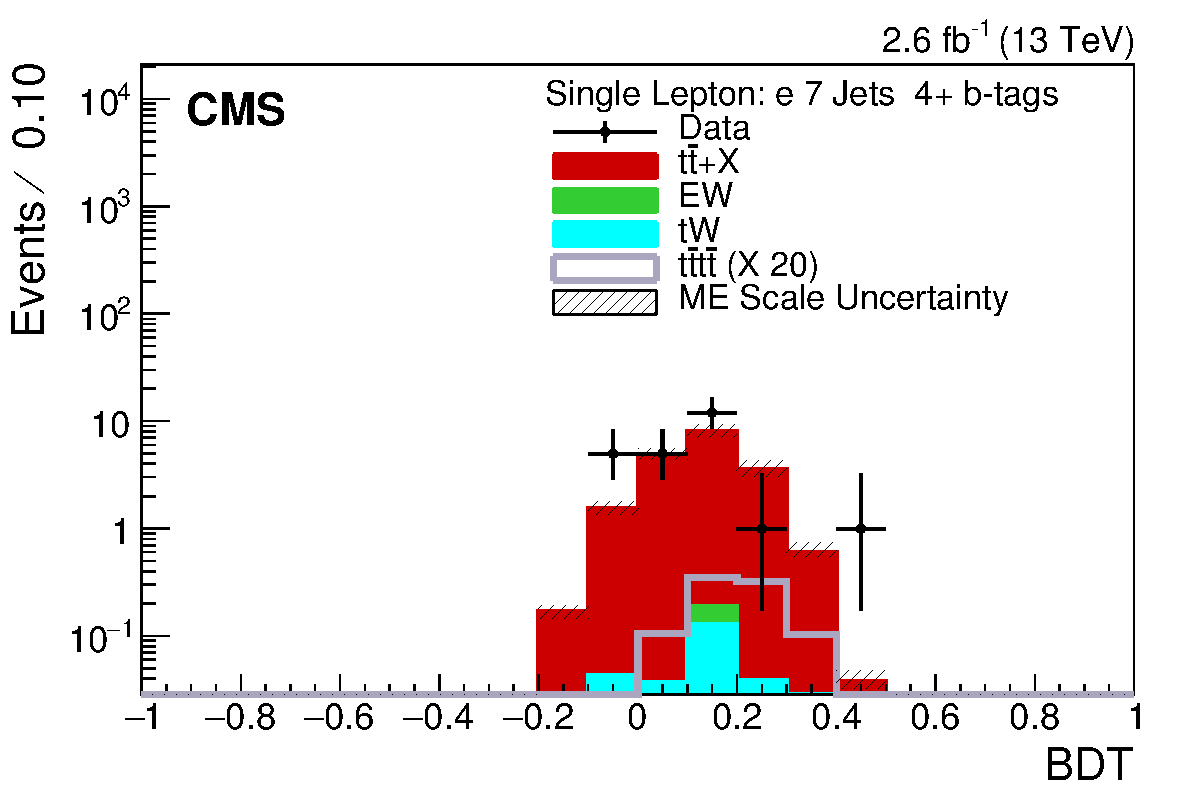
\includegraphics[width=0.48\textwidth]{images/Run2/BDT_El29Aug400trees_5MinNodeSize_20nCuts_3MaxDepth_5adaboostbeta_adaBoost_alphaSTune_noMinEvents7nJets4nMtags_StackLogY.pdf}
    \caption{The BDT output distributions for AdaBoost for data and simulation in the $\mu$ + jets channel (left) and e + jets channel (right) are shown for the 7 \njets and $\geq4$ \nMtags category.}
    \label{fig:BDT_Mu29Aug400trees_5MinNodeSize_20nCuts_3MaxDepth_5adaboostbeta_adaBoost_alphaSTune_noMinEvents74}
\end{figure}

\begin{figure}[ht!]
    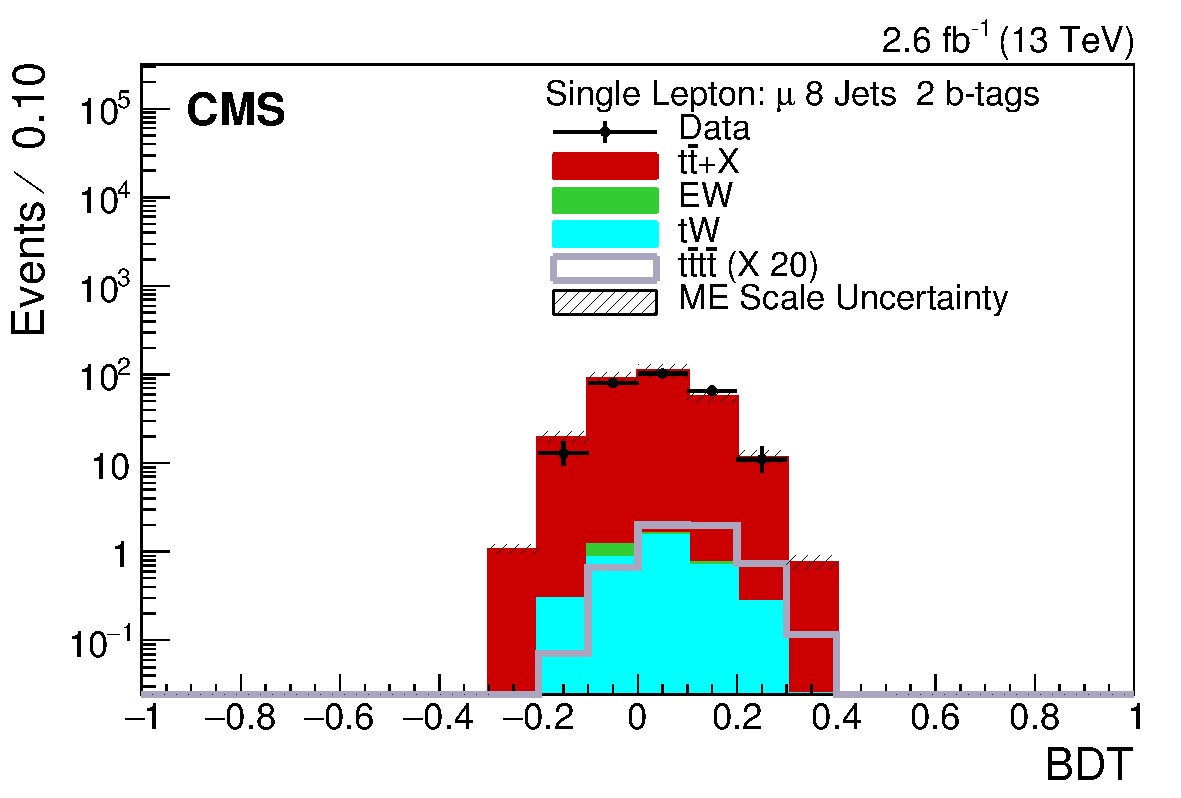
\includegraphics[width=0.48\textwidth]{images/Run2/BDT_Mu29Aug400trees_5MinNodeSize_20nCuts_3MaxDepth_5adaboostbeta_adaBoost_alphaSTune_noMinEvents8nJets2nMtags_StackLogY.pdf}
    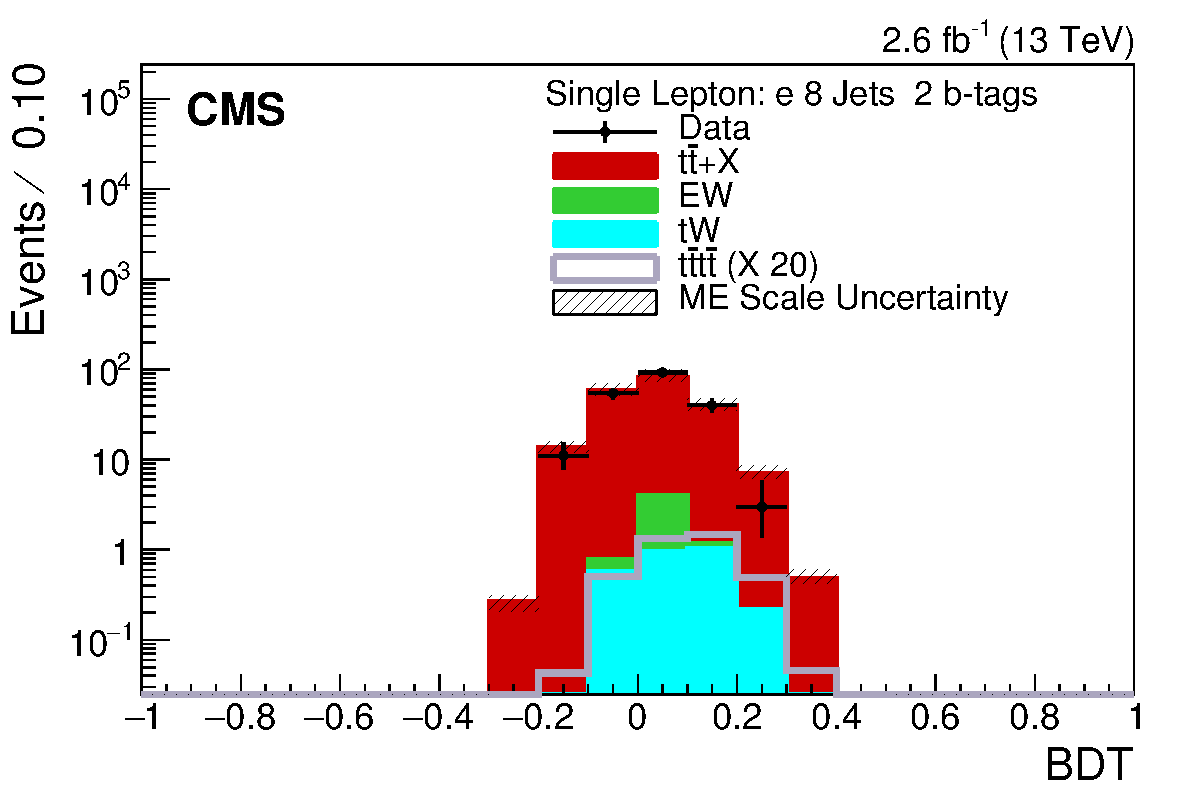
\includegraphics[width=0.48\textwidth]{images/Run2/BDT_El29Aug400trees_5MinNodeSize_20nCuts_3MaxDepth_5adaboostbeta_adaBoost_alphaSTune_noMinEvents8nJets2nMtags_StackLogY.pdf} 
    \caption{The BDT output distributions for AdaBoost for data and simulation in the $\mu$ + jets channel (left) and $e$ + jets channel (left) are shown for the 8 \njets and 2 \nMtags category.}
    \label{fig:BDT_Mu29Aug400trees_5MinNodeSize_20nCuts_3MaxDepth_5adaboostbeta_adaBoost_alphaSTune_noMinEvents82}
\end{figure}

\begin{figure}[ht!]
    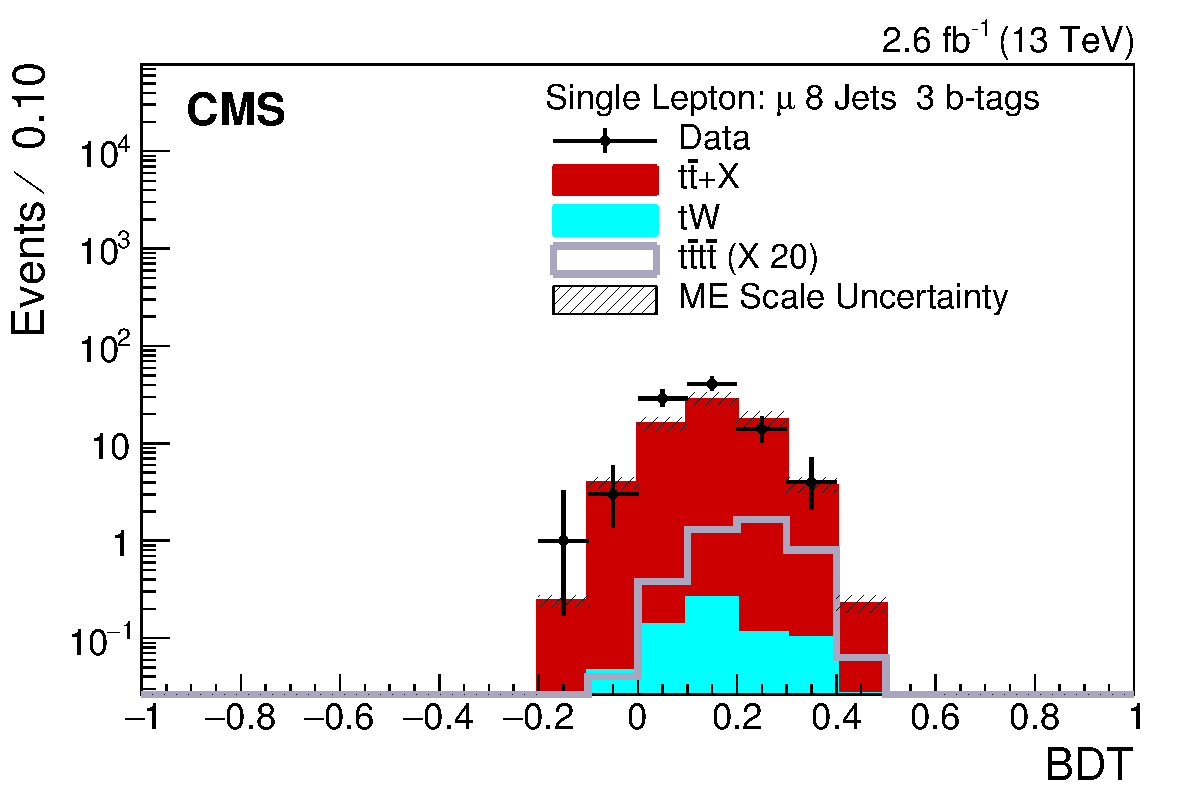
\includegraphics[width=0.48\textwidth]{images/Run2/BDT_Mu29Aug400trees_5MinNodeSize_20nCuts_3MaxDepth_5adaboostbeta_adaBoost_alphaSTune_noMinEvents8nJets3nMtags_StackLogY.pdf}
    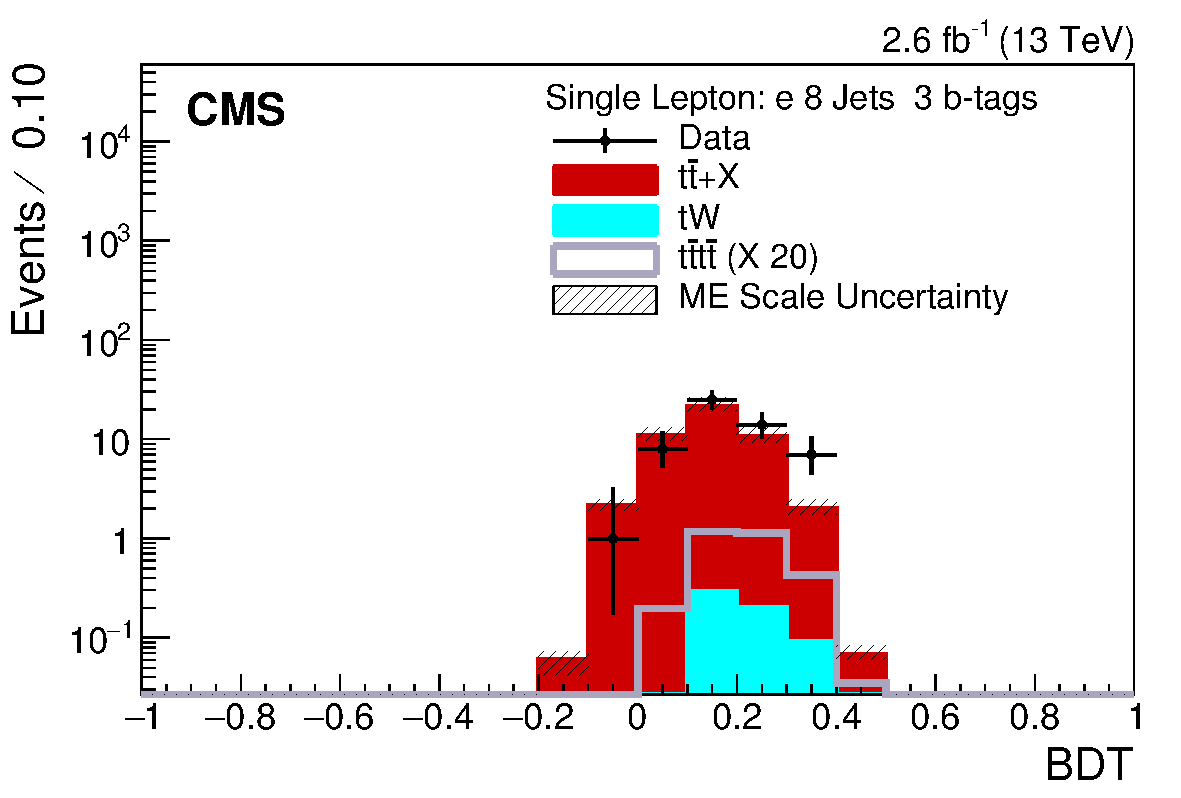
\includegraphics[width=0.48\textwidth]{images/Run2/BDT_El29Aug400trees_5MinNodeSize_20nCuts_3MaxDepth_5adaboostbeta_adaBoost_alphaSTune_noMinEvents8nJets3nMtags_StackLogY.pdf} 
    \caption{The BDT output distributions for AdaBoost for data and simulation in the $\mu$ + jets channel (left) and $e$ + jets channel (left) are shown for the 8 \njets category and 3 \nMtags category.}
    \label{fig:BDT_Mu29Aug400trees_5MinNodeSize_20nCuts_3MaxDepth_5adaboostbeta_adaBoost_alphaSTune_noMinEvents83}
\end{figure}


\begin{figure}[ht!]
    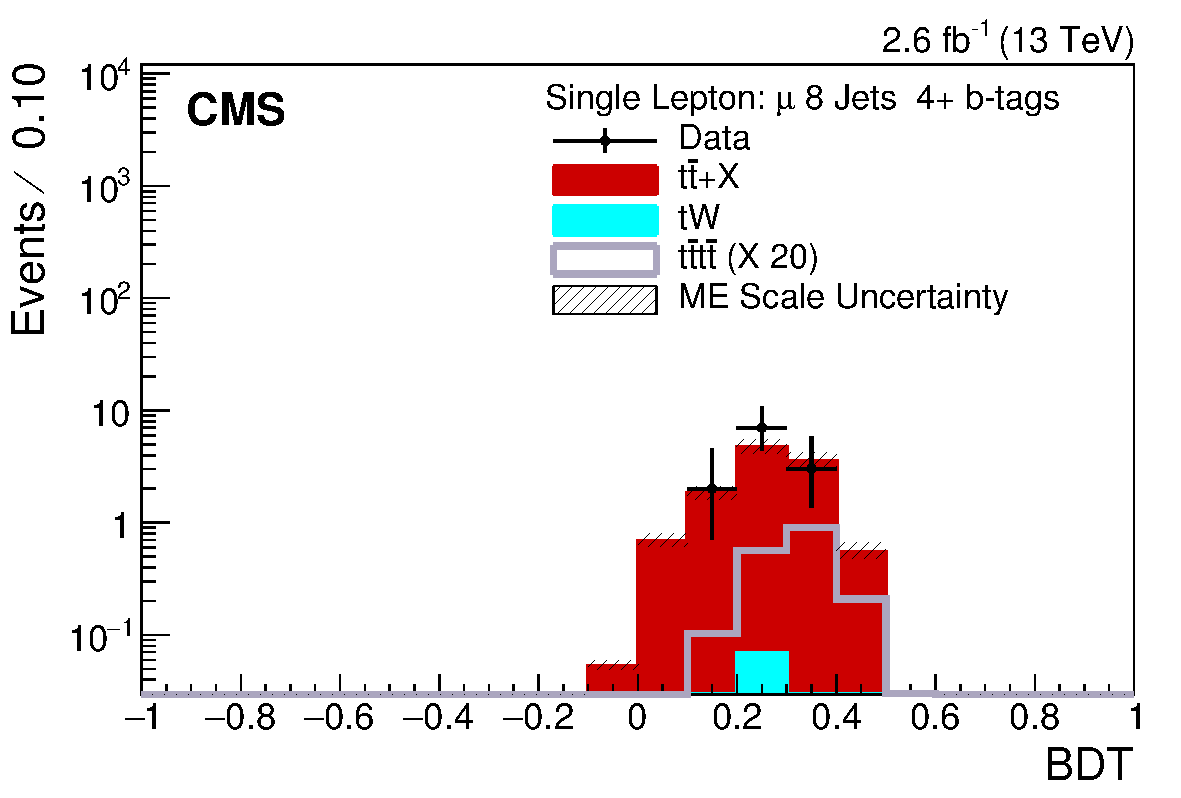
\includegraphics[width=0.48\textwidth]{images/Run2/BDT_Mu29Aug400trees_5MinNodeSize_20nCuts_3MaxDepth_5adaboostbeta_adaBoost_alphaSTune_noMinEvents8nJets4nMtags_StackLogY.pdf}
    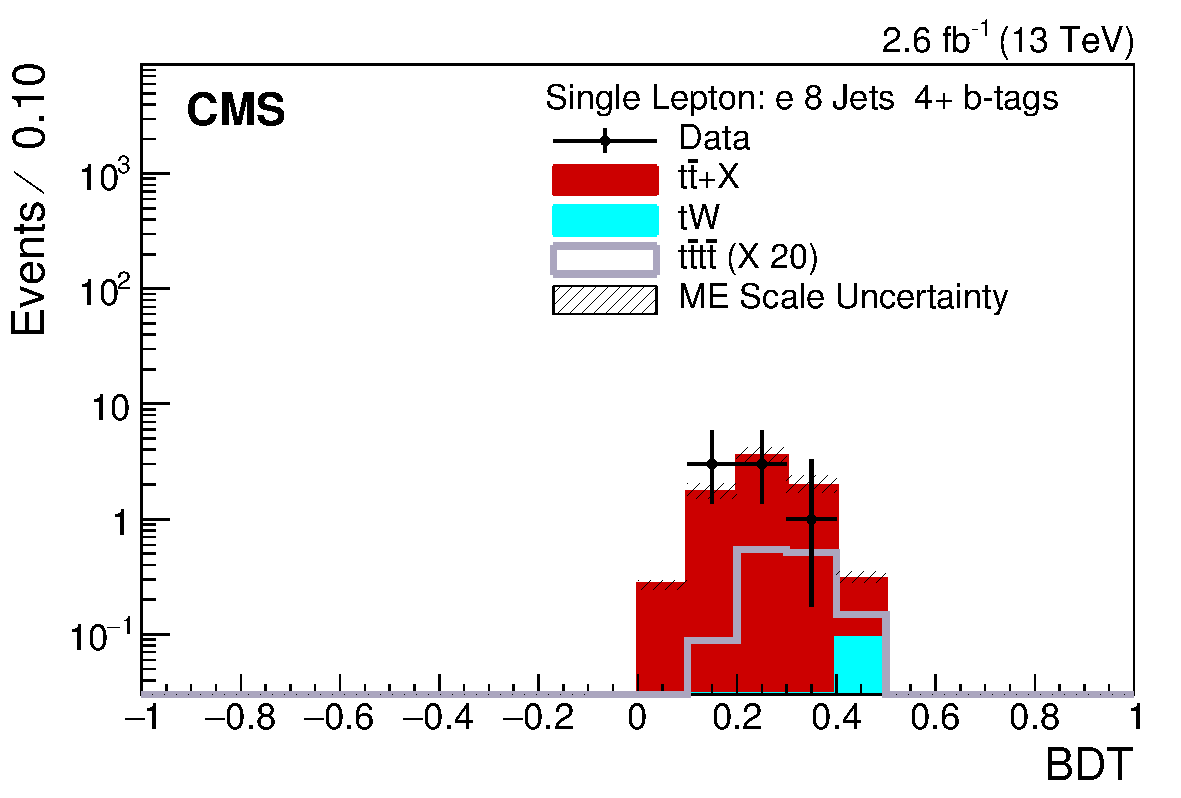
\includegraphics[width=0.48\textwidth]{images/Run2/BDT_El29Aug400trees_5MinNodeSize_20nCuts_3MaxDepth_5adaboostbeta_adaBoost_alphaSTune_noMinEvents8nJets4nMtags_StackLogY.pdf}
    \caption{The BDT output distributions for AdaBoost for data and simulation in the $\mu$ + jets channel (left) and $e$ + jets channel (right) are shown for the 8 \njets and $\geq4$ \nMtags category.}
    \label{fig:BDT_Mu29Aug400trees_5MinNodeSize_20nCuts_3MaxDepth_5adaboostbeta_adaBoost_alphaSTune_noMinEvents84}
\end{figure}

\begin{figure}[ht!]
    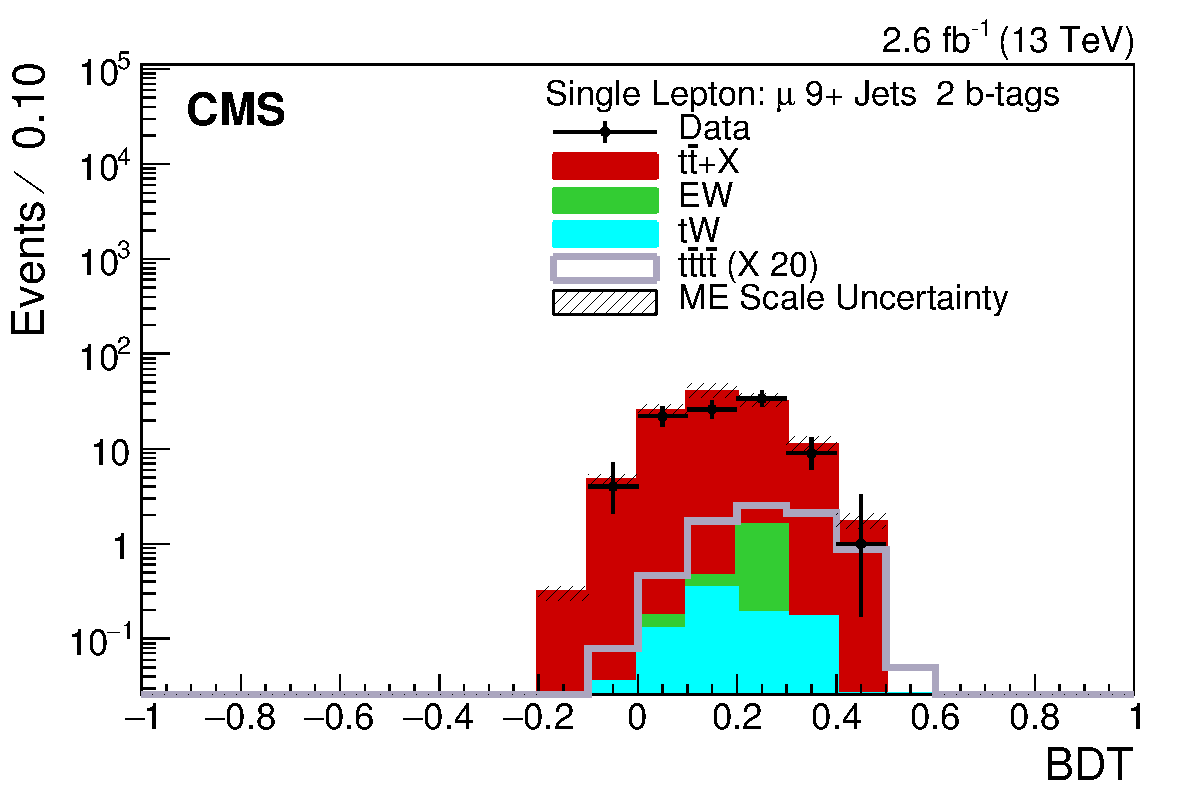
\includegraphics[width=0.48\textwidth]{images/Run2/BDT_Mu29Aug400trees_5MinNodeSize_20nCuts_3MaxDepth_5adaboostbeta_adaBoost_alphaSTune_noMinEvents9nJets2nMtags_StackLogY.pdf}
    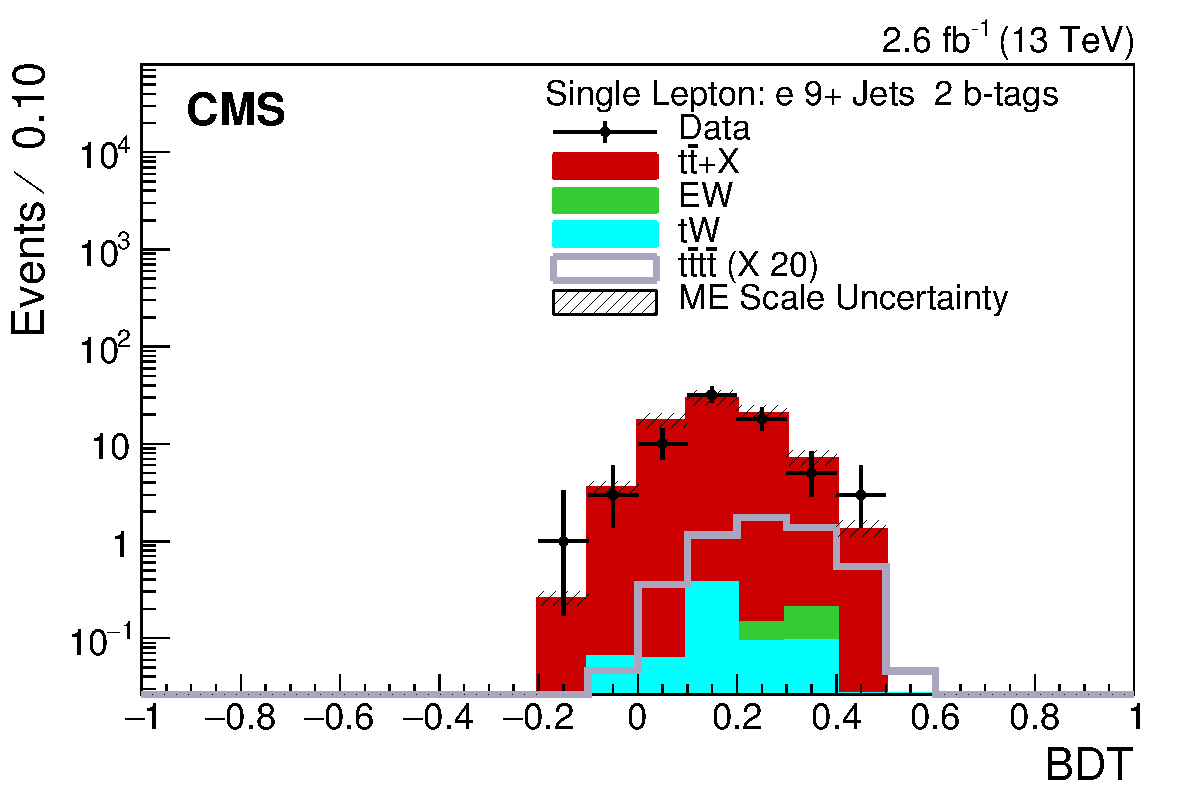
\includegraphics[width=0.48\textwidth]{images/Run2/BDT_El29Aug400trees_5MinNodeSize_20nCuts_3MaxDepth_5adaboostbeta_adaBoost_alphaSTune_noMinEvents9nJets2nMtags_StackLogY.pdf} 
    \caption{The BDT output distributions for AdaBoost for data and simulation in the $\mu$ + jets channel (left) and $e$ + jets channel (left) are shown for the $\geq9$ \njets  and 2 \nMtags category.}
    \label{fig:BDT_Mu29Aug400trees_5MinNodeSize_20nCuts_3MaxDepth_5adaboostbeta_adaBoost_alphaSTune_noMinEvents92}
\end{figure}


\section{Systematic shape studies \label{app:sysshapes}}

In this section the alternative BDT distribution shapes are examined for a few of the shape systematic described in Section~\ref{sec:uncertainties13}. The largest systematic uncertainties are the JES, ME scale systematics and the \ttbar generator choice. The JER and PU up/down (red/cyan) shapes deviate very little from the nominal distributions (blue). In \ttbar there are several distributions including JER and PU systematics show relatively flat behaviour with respect to the nominal distribution and in future analyses could be considered for incorporation into a normalisation systematic uncertainty.

% \begin{figure}[ht!]
%     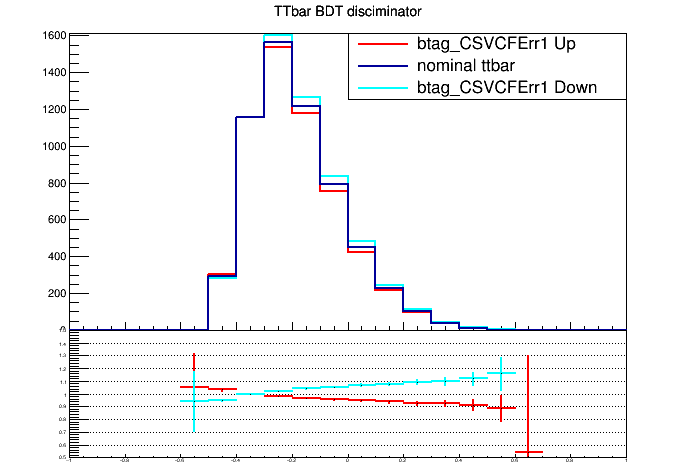
\includegraphics[width=0.48\textwidth]{images/Run2/Sys/btag_CSVCFErr1systt.png}
%     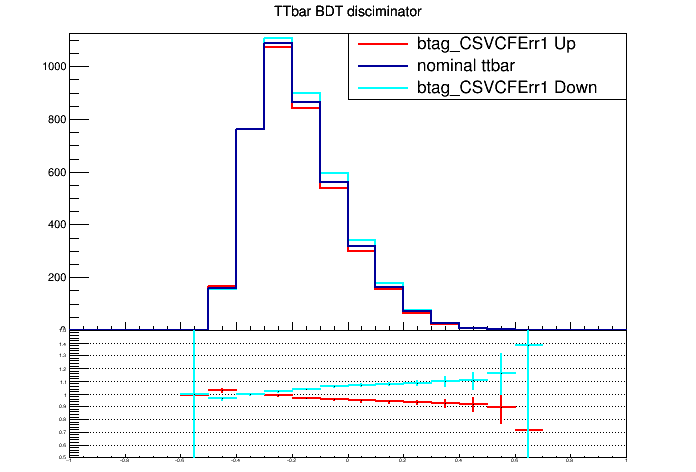
\includegraphics[width=0.48\textwidth]{images/Run2/Sys/btag_CSVCFErr1systt_e.png}     
%     \caption{The BDT shapes for b-tag event-weight for linear charm flavour systematic in \ttbar for the $\mu$ + jets channel (left) and e + jets channel (right).}
%     \label{fig:SysShapesCFErrtt1}
% \end{figure}
% \begin{figure}[ht!]
%     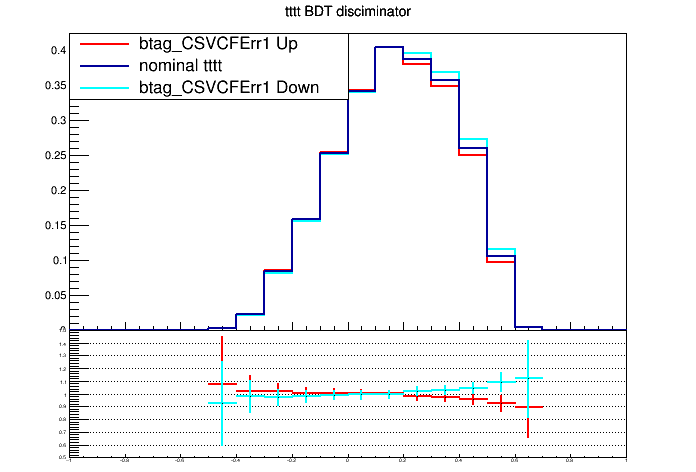
\includegraphics[width=0.48\textwidth]{images/Run2/Sys/btag_CSVCFErr1systttt.png}
%     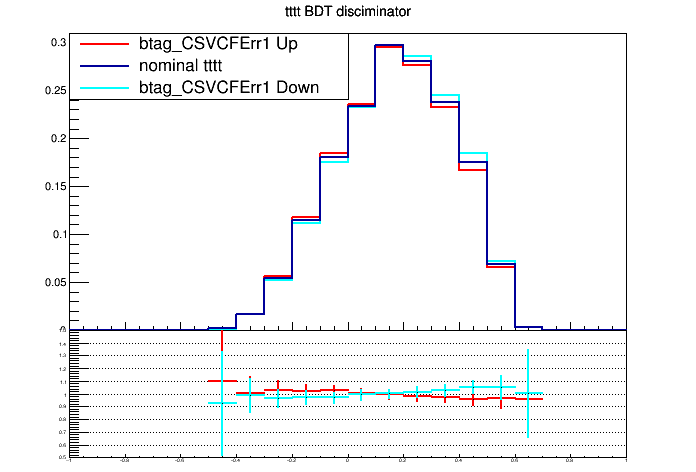
\includegraphics[width=0.48\textwidth]{images/Run2/Sys/btag_CSVCFErr1systttt_e.png}     
%     \caption{The BDT shapes for b-tag event-weight for linear charm flavour systematic in \tttt for the $\mu$ + jets channel (left) and e + jets channel (right).}
%     \label{fig:SysShapesCFErrtttt1}
% \end{figure}
% \begin{figure}[ht!]
%     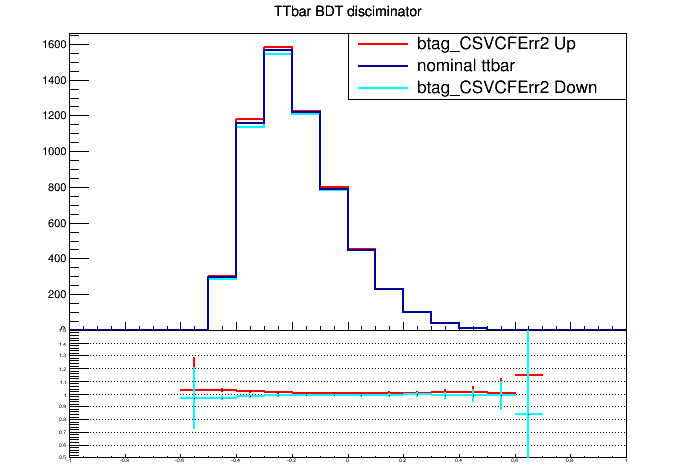
\includegraphics[width=0.48\textwidth]{images/Run2/Sys/btag_CSVCFErr2systt.png}
%     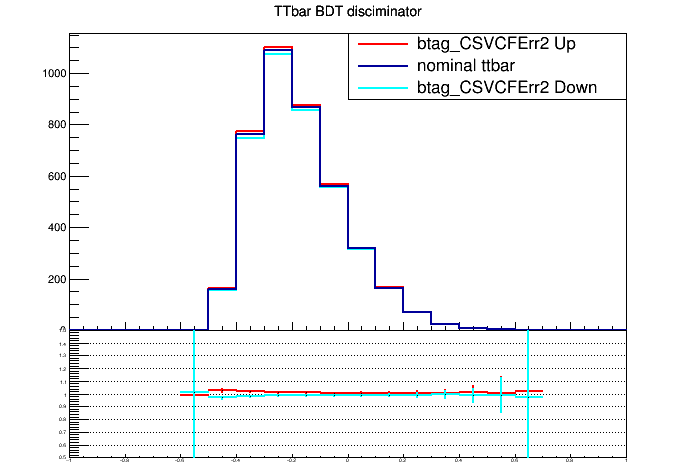
\includegraphics[width=0.48\textwidth]{images/Run2/Sys/btag_CSVCFErr2systt_e.png}     
%     \caption{The BDT shapes for b-tag event-weight for quadratic charm flavour systematic in \ttbar for the $\mu$ + jets channel (left) and e + jets channel (right).}
%     \label{fig:SysShapesCFErrtt2}
% \end{figure}

% \begin{figure}[ht!]
%     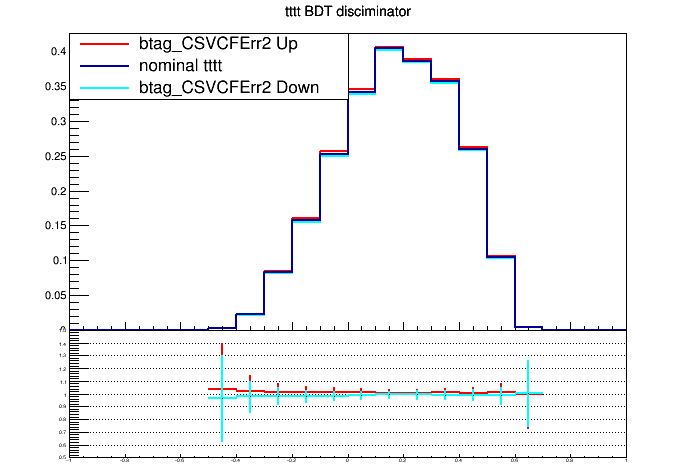
\includegraphics[width=0.48\textwidth]{images/Run2/Sys/btag_CSVCFErr2systttt.png}
%     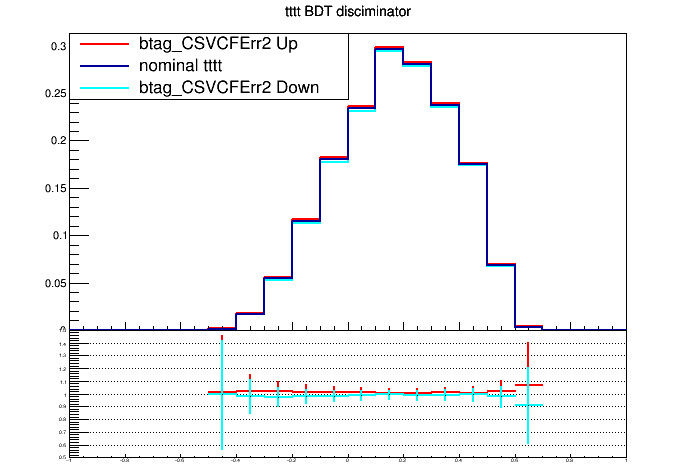
\includegraphics[width=0.48\textwidth]{images/Run2/Sys/btag_CSVCFErr2systttt_e.png}     
%     \caption{The BDT shapes for b-tag event-weight for quadratic charm flavour systematic in \tttt for the $\mu$ + jets channel (left) and e + jets channel (right).}
%     \label{fig:SysShapesCFErrtttt2}
% \end{figure}
% \begin{figure}[ht!]
%     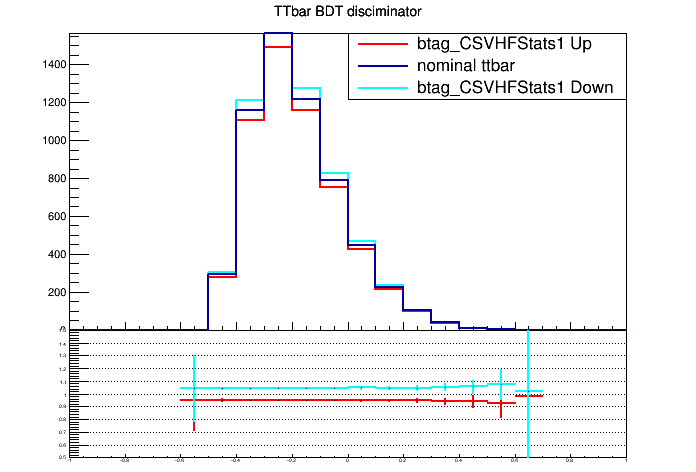
\includegraphics[width=0.48\textwidth]{images/Run2/Sys/btag_CSVHFStats1systt.png}
%     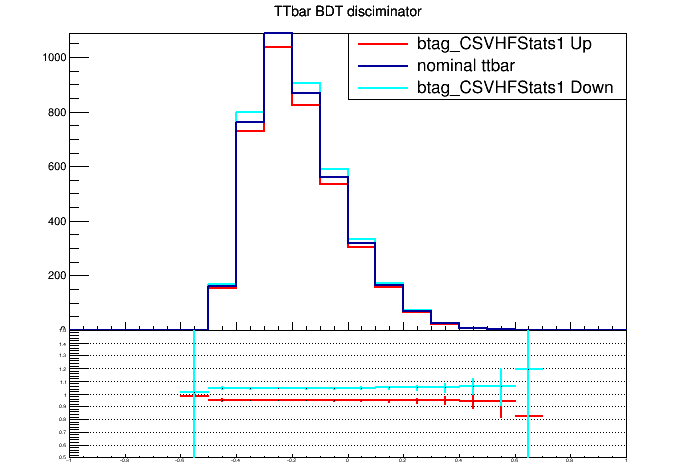
\includegraphics[width=0.48\textwidth]{images/Run2/Sys/btag_CSVHFStats1systt_e.png}     
%     \caption{The BDT shapes for b-tag event-weight for linear heavy flavour systematic in \ttbar for the $\mu$ + jets channel (left) and e + jets channel (right).}
%     \label{fig:SysShapesHFStatstt1}
% \end{figure}
% \begin{figure}[ht!]
%     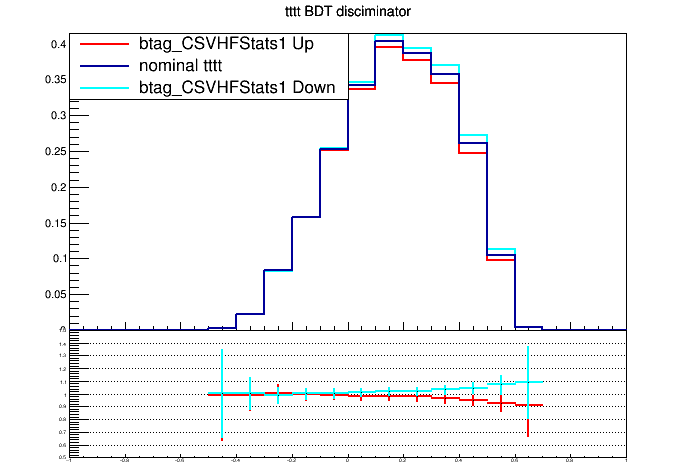
\includegraphics[width=0.48\textwidth]{images/Run2/Sys/btag_CSVHFStats1systttt.png}
%     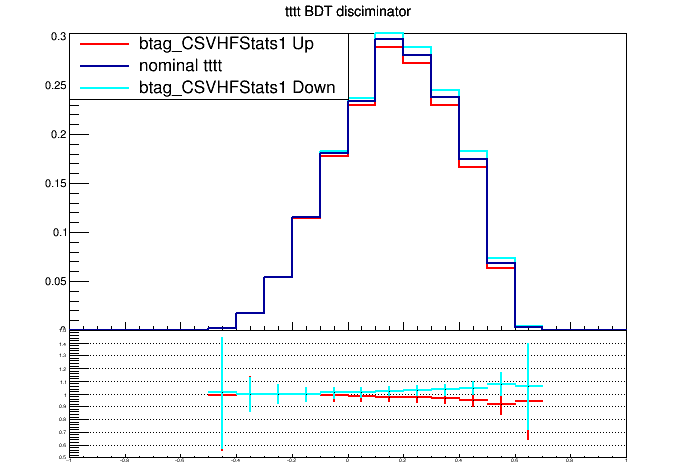
\includegraphics[width=0.48\textwidth]{images/Run2/Sys/btag_CSVHFStats1systttt_e.png}     
%     \caption{The BDT shapes for b-tag event-weight for linear heavy flavour systematic in \tttt for the $\mu$ + jets channel (left) and e + jets channel (right).}
%     \label{fig:SysShapesHFStatstttt1}
% \end{figure}

% \begin{figure}[ht!]
%     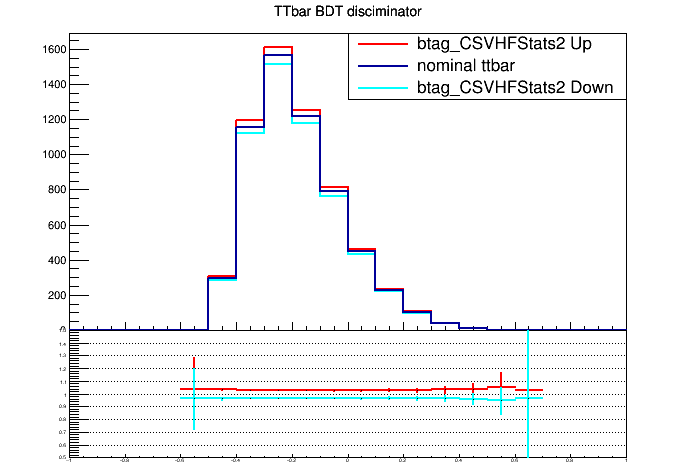
\includegraphics[width=0.48\textwidth]{images/Run2/Sys/btag_CSVHFStats2systt.png}
%     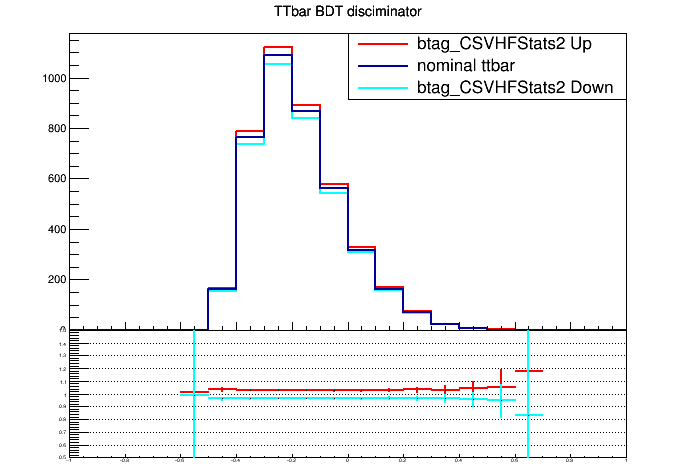
\includegraphics[width=0.48\textwidth]{images/Run2/Sys/btag_CSVHFStats2systt_e.png}     
%     \caption{The BDT shapes for b-tag event-weight for quadratic heavy flavour systematic in \ttbar for the $\mu$ + jets channel (left) and e + jets channel (right).}
%     \label{fig:SysShapesHFStatstt2}
% \end{figure}
% \begin{figure}[ht!]
%     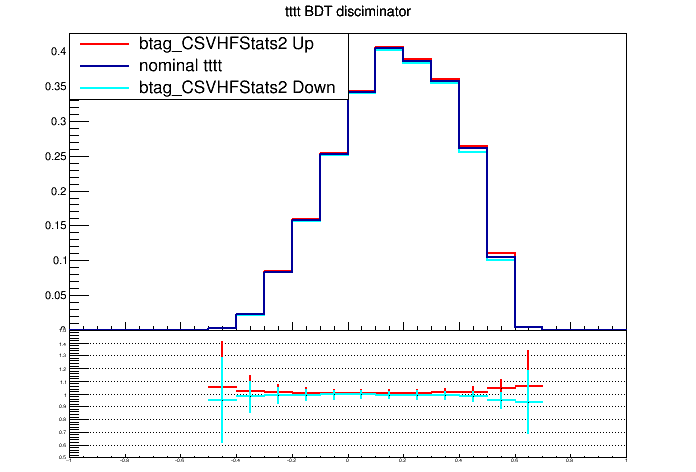
\includegraphics[width=0.48\textwidth]{images/Run2/Sys/btag_CSVHFStats2systttt.png}
%     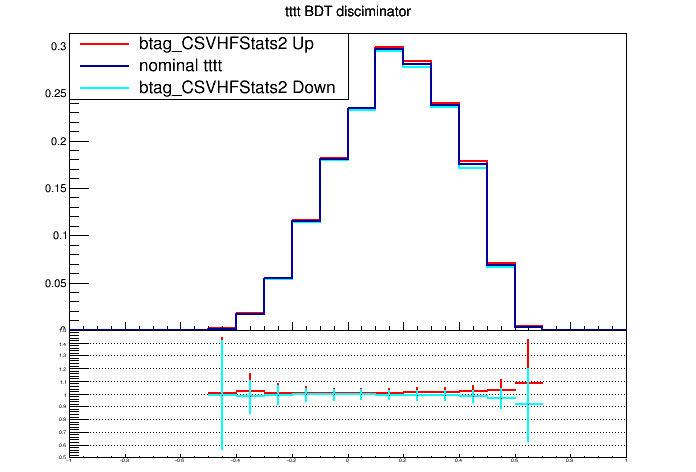
\includegraphics[width=0.48\textwidth]{images/Run2/Sys/btag_CSVHFStats2systttt_e.png}     
%     \caption{The BDT shapes for b-tag event-weight for quadratic heavy flavour systematic in \tttt for the $\mu$ + jets channel (left) and e + jets channel (right).}
%     \label{fig:SysShapesHFStatstttt2}
% \end{figure}
% \begin{figure}[ht!]
%     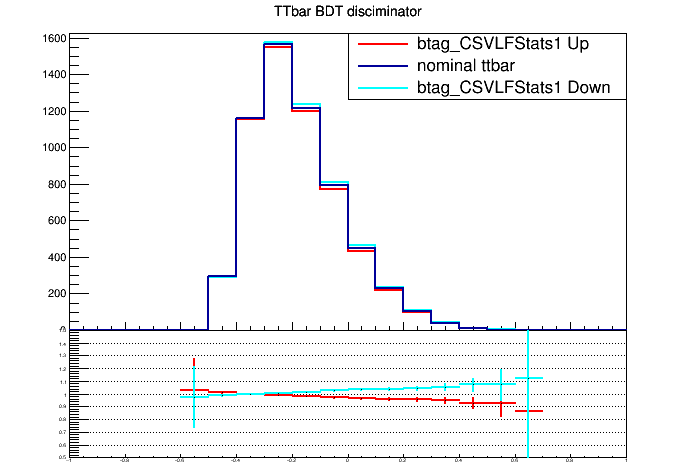
\includegraphics[width=0.48\textwidth]{images/Run2/Sys/btag_CSVLFStats1systt.png}
%     \includegraphics[width=0.48\textwidth]{images/Run2/Sys/btag_CSVLFStats1systt_e.png}     
%     \caption{The BDT shapes for b-tag event-weight for linear light flavour systematic in \ttbar for the $\mu$ + jets channel (left) and e + jets channel (right).}
%     \label{fig:SysShapesLStatstt1}
% \end{figure}

% \begin{figure}[ht!]
%     \includegraphics[width=0.48\textwidth]{images/Run2/Sys/btag_CSVLFStats1systttt.png}
%     \includegraphics[width=0.48\textwidth]{images/Run2/Sys/btag_CSVLFStats1systttt_e.png}     
%     \caption{The BDT shapes for b-tag event-weight for linear light flavour systematic in \tttt for the $\mu$ + jets channel (left) and e + jets channel (right).}
%     \label{fig:SysShapesLStatstttt1}
% \end{figure}
% \begin{figure}[ht!]
%     \includegraphics[width=0.48\textwidth]{images/Run2/Sys/btag_CSVLFStats2systt.png}
%     \includegraphics[width=0.48\textwidth]{images/Run2/Sys/btag_CSVLFStats2systt_e.png}     
%     \caption{The BDT shapes for b-tag event-weight for quadratic light flavour systematic in \ttbar for the $\mu$ + jets channel (left) and e + jets channel (right).}
%     \label{fig:SysShapesLStatstttt2}
% \end{figure}
% \begin{figure}[ht!]
%     \includegraphics[width=0.48\textwidth]{images/Run2/Sys/btag_CSVLFStats2systttt.png}
%     \includegraphics[width=0.48\textwidth]{images/Run2/Sys/btag_CSVLFStats2systttt_e.png}     
%     \caption{The BDT shapes for b-tag event-weight for quadratic light flavour systematic in \tttt for the $\mu$ + jets channel (left) and e + jets channel (right).}
%     \label{fig:SysShapesLStatstt2}
% \end{figure}

% \begin{figure}[ht!]
%     \includegraphics[width=0.48\textwidth]{images/Run2/Sys/btag_CSVHFsystt.png}
%     \includegraphics[width=0.48\textwidth]{images/Run2/Sys/btag_CSVHFsystt_e.png}     
%     \caption{The BDT shapes for b-tag event-weight for heavy flavour contamination of light jets in \ttbar for the $\mu$ + jets channel (left) and e + jets channel (right).}
%     \label{fig:SysShapesHFsystt}
% \end{figure}
% \begin{figure}[ht!]
%     \includegraphics[width=0.48\textwidth]{images/Run2/Sys/btag_CSVHFsystttt.png}
%     \includegraphics[width=0.48\textwidth]{images/Run2/Sys/btag_CSVHFsystttt_e.png}     
%     \caption{The BDT shapes for b-tag event-weight for heavy flavour contamination of light jets in \tttt for the $\mu$ + jets channel (left) and e + jets channel (right).}
%     \label{fig:SysShapesHFsystttt}
% \end{figure}
% \begin{figure}[ht!]
%     \includegraphics[width=0.48\textwidth]{images/Run2/Sys/btag_CSVLFsystt.png}
%     \includegraphics[width=0.48\textwidth]{images/Run2/Sys/btag_CSVLFsystt_e.png}     
%     \caption{The BDT shapes for b-tag event-weight for light flavour contamination of heavy jets in \ttbar for the $\mu$ + jets channel (left) and e + jets channel (right).}
%     \label{fig:SysShapesLFsystt}
% \end{figure}

% \begin{figure}[ht!]
%     \includegraphics[width=0.48\textwidth]{images/Run2/Sys/btag_CSVLFsystttt.png}
%     \includegraphics[width=0.48\textwidth]{images/Run2/Sys/btag_CSVLFsystttt_e.png}     
%     \caption{The BDT shapes for b-tag event-weight for light flavour contamination of heavy jets in \tttt for the $\mu$ + jets channel (left) and e + jets channel (right).}
%     \label{fig:SysShapesLFsystttt}
% \end{figure}


\begin{figure}[ht!]
    \includegraphics[width=0.48\textwidth]{images/Run2/Sys/JERsystt.pdf}
    \includegraphics[width=0.48\textwidth]{images/Run2/Sys/JERsystt_e.pdf}     
    \caption{The BDT shapes for JER systematic in \ttbar for the $\mu$ + jets channel (left) and e + jets channel (right).}
    \label{fig:SysShapesJERtt}
\end{figure}

% \begin{figure}[ht!]
%     \includegraphics[width=0.48\textwidth]{images/Run2/Sys/JERsystttt.pdf}
%     \includegraphics[width=0.48\textwidth]{images/Run2/Sys/JERsystttt_e.pdf}     
%     \caption{The BDT shapes for JER systematic in \tttt for the $\mu$ + jets channel (left) and e + jets channel (right).}
%     \label{fig:SysShapesJERtttt}
% \end{figure}

\begin{figure}[ht!]
    \includegraphics[width=0.48\textwidth]{images/Run2/Sys/JESsystt.pdf}
    \includegraphics[width=0.48\textwidth]{images/Run2/Sys/JESsystt_e.pdf}     
    \caption{The BDT shapes for JES systematic in \ttbar for the $\mu$ + jets channel (left) and e + jets channel (right).}
    \label{fig:SysShapesJEStt}
\end{figure}

\begin{figure}[ht!]
    \includegraphics[width=0.48\textwidth]{images/Run2/Sys/JESsystttt.pdf}
    \includegraphics[width=0.48\textwidth]{images/Run2/Sys/JESsystttt_e.pdf}     
    \caption{The BDT shapes for JES systematic in \tttt for the $\mu$ + jets channel (left) and e + jets channel (right).}
    \label{fig:SysShapesJEStttt}
\end{figure}

\begin{figure}[ht!]
    \includegraphics[width=0.48\textwidth]{images/Run2/Sys/MEScalesystt.pdf}
    \includegraphics[width=0.48\textwidth]{images/Run2/Sys/MEScalesystt_e.pdf}     
    \caption{The BDT shapes for ME scale systematic in \ttbar for the $\mu$ + jets channel (left) and e + jets channel (right).}
    \label{fig:SysShapesMEtt}
\end{figure}
\begin{figure}[ht!]
    \includegraphics[width=0.48\textwidth]{images/Run2/Sys/MEScalesystttt.pdf}
    \includegraphics[width=0.48\textwidth]{images/Run2/Sys/MEScalesystttt_e.pdf}     
    \caption{The BDT shapes for ME scale systematic in \tttt for the $\mu$ + jets channel (left) and e + jets channel (right).}
    \label{fig:SysShapesMEtttt}
\end{figure}

\begin{figure}[ht!]
    \includegraphics[width=0.48\textwidth]{images/Run2/Sys/PUsystt.pdf} 
    \includegraphics[width=0.48\textwidth]{images/Run2/Sys/PUsystt_e.pdf}     
    \caption{The BDT shapes for PU systematic in \ttbar for the $\mu$ + jets channel (left) and e + jets channel (right).}
    \label{fig:SysShapesPUtt}
\end{figure}

% \begin{figure}[ht!]
%     \includegraphics[width=0.48\textwidth]{images/Run2/Sys/PUsystttt.pdf} 
%     \includegraphics[width=0.48\textwidth]{images/Run2/Sys/PUsystttt_e.pdf}     
%     \caption{The BDT shapes for PU systematic in \tttt for the $\mu$ + jets channel (left) and e + jets channel (right).}
%     \label{fig:SysShapesPUtttt}
% \end{figure}

% \begin{figure}[ht!]
%     \includegraphics[width=0.48\textwidth]{images/Run2/Sys/ScaleHsystt.pdf}
%     \includegraphics[width=0.48\textwidth]{images/Run2/Sys/ScaleHsystt_e.pdf}     
%     \caption{The BDT shapes for hadronisation scale systematic in \ttbar for the $\mu$ + jets channel (left) and e + jets channel (right).}
%     \label{fig:SysShapesScaleHtt}
% \end{figure}

\begin{figure}[ht!]
    \includegraphics[width=0.48\textwidth]{images/Run2/Sys/ttGeneratorsystt.pdf}
    \includegraphics[width=0.48\textwidth]{images/Run2/Sys/ttGeneratorsystt_e.pdf}     
    \caption{The BDT shapes for ttGenerator choice systematic in \ttbar for the $\mu$ + jets channel (left) and e + jets channel (right).}
    \label{fig:SysShapesttGen}
\end{figure}


\subsection{Studies of impact of systematic uncertainties \label{app:sysminusone}}

The impact of each systematic uncertainty on the expected limit is shown in Table~\ref{tab:sysRemoved} by removing each systematic from the fit and recalculating the expected limit. The systematic uncertainties which have the largest impact are the \ttbar ME scale, \ttbar PS scale and the JES scale, which is applied to both \ttbar and \tttt. The \ttbar ME scale has a large impact on the modelling of the signal process whereas the \ttbar PS scale has a big effect on the modelling of the additional jets produced in high jet multiplicity \ttbar events which pass the baseline event selection.

\begin{table}[ht]
\centering
\caption{Expected limits on \tttt production which each systematic removed in turn}
\label{tab:sysRemoved}
\begin{tabular}{|l|l|}
\hline
% \rule{0pt}{4ex}    
% \rule[-1.2ex]{0pt}{0pt}
Systematic uncertainty removed & Expected limit ($\times$\sigmattttsm) \T \B\\ 
% \rule{0pt}{4ex}    

\hline
None                           & 16.0000                                                         \\ \hline
\ttbar ME scale                & 16.0625                                                         \\ \hline
\tttt ME scale                 & 14.4375                                                         \\ \hline
JER                            & 15.9375                                                         \\ \hline
JES                            & 15.3125                                                         \\ \hline
PS scale                       & 15.0625                                                         \\ \hline
PU                             & 16.0625                                                         \\ \hline
Generator uncertainty          & 15.9531                                                         \\ \hline
\ttbar heavy flav              & 15.5625                                                         \\ \hline
Luminosity                     & 16.0625                                                         \\ \hline
Lepton SF Mu                   & 16.0625                                                         \\ \hline
Lepton SF El                   & 15.9062                                                         \\ \hline
\ttbar norm                    & 16.0000                                                         \\ \hline
\tttt norm                     & 15.9062                                                         \\ \hline
EW norm                        & 16.0000                                                         \\ \hline
Single top norm                & 16.0000                                                         \\ \hline
% b-tag light SF                 & 12.5625                                                         \\ \hline
btagWeightCSVCFErr1            & 16.0625                                                         \\ \hline
btagWeightCSVCFErr2            & 16.0625                                                         \\ \hline
btagWeightCSVHF                & 15.5625                                                         \\ \hline
btagWeightCSVHFStats1          & 15.9375                                                         \\ \hline
btagWeightCSVHFStats2          & 15.9531                                                         \\ \hline
btagWeightCSVLF                & 15.9375                                                         \\ \hline
btagWeightCSVLFStats1          & 16.0625                                                         \\ \hline
btagWeightCSVLFStats2          & 15.9062                                                         \\ \hline
\end{tabular}
\end{table}


\section{Correlation matrices for fit nuisance parameters \label{app:corrFit}}


The correlation matrix for the fit nuisance parameters in the background only scenario can be see in Fig.~\ref{fig:FitCorr}. There is some correlation between the various b-tagging scale factors and also a correlation between the heavy flavour \heavyflavourone / \heavyflavourtwo modelling and the \ttbar ME scale, where the \heavyflavourone / \heavyflavourtwo is expected to be related to the choice of ME scale.

\begin{figure}[ht!]
    \includegraphics[width=0.9\textwidth]{images/Run2/FitCorr.pdf}
    \caption{The correlation matrices for background only for the fit parameters.}
    \label{fig:FitCorr}
\end{figure}
